\documentclass[11pt, a4paper]{book}
% -----------------------------------------------------------------------------------
% For every instance of this template, change the following:
%	> Title Page information starting at line 57;
%	> Summary of Part on line 113
%	> Input file on line 122;
%	> Reference file on line 125;
%	> Glossary file on line 128;
% -----------------------------------------------------------------------------------
\usepackage{fancyhdr}
\pagestyle{fancy}
\fancyhf{}

\usepackage[english]{babel}
\usepackage{graphicx}
\usepackage[colorlinks,hyperindex,plainpages=false,breaklinks]{hyperref}
\usepackage{amssymb}
\usepackage{wasysym} 
\usepackage{wrapfig}
\usepackage{enumerate}
\usepackage{placeins} % Necessary for \FloatBarrier
\usepackage{subfig}   % Necessary for subfloat (images next to each other)
\usepackage{color}
\usepackage[usenames,dvipsnames,svgnames]{xcolor}
\usepackage{listings}
\usepackage{fancyhdr}

\definecolor{codelightgray}{rgb}{0.87,0.87,0.87}

\hypersetup{colorlinks=true,% 
	linkcolor=black,%
	citecolor=red,%
	filecolor=blue,% 
	menucolor=black,% 
	pagecolor=black,%
	urlcolor=black}
	
\lstset{language=,
    keywordstyle=\color{blue},
    basicstyle=\scriptsize\ttfamily,
    showstringspaces=false,
    backgroundcolor=\color{codelightgray},
    morekeywords={SELECT,FROM,WHERE,AND,OR,EClass}
}

\newcommand{\note}[1]{\marginpar{\emph{#1}}}

\setcounter{tocdepth}{2}

\setlength{\parindent}{0pt} 
\setlength{\parskip}{0.3cm}


% --- Add Path to find all relevant files; avoids having to type in full path
% \graphicspath{{../../00_introduction/common/}{../installation_images/}}
\graphicspath{{../00_introduction/common/}{installation_images/}{03_simpleDemo/03_sectionImages/}}
 
% Remove section numbers 0.1, 0.2 ..
\renewcommand{\thesection}{\arabic{section}} 
 
% --- Title Page Information
\def\partTitle{Part I: Installation \& Set-up}
\def\versionNumber{3.4}
\title{
\flushright
{\LARGE\bfseries An Introduction to Metamodelling\\
and Graph Transformations}
\noindent\rule[-1ex]{\textwidth}{5pt}\\[2.5ex]
\hfill\emph{\LARGE\bfseries with eMoflon}
\flushleft
{\small Version 2.1}
\flushright

\includegraphics[width=0.85\textwidth]{pics/eMoflon3} 
}

\date{}  
\author{} 

% --- HEADER FUNCTIONS --------------------------------------------------------------
% Default plain header; turn off all lines and colors
\newcommand{\noHeader}{
	\fancyhead[OR]{\thepage}
	\fancyhead[EL]{\thepage}
	\renewcommand{\headrulewidth}{0pt}
}

% General Header for when instructions overlap
\newcommand{\genHeader}{
	\fancyhead[OR]{\thepage}
	\fancyhead[EL]{\thepage}
	\renewcommand{\headrulewidth}{1.5pt}
 	\renewcommand{\headrule}{\hbox to\headwidth{%
  		\color{Black}\leaders\hrule height \headrulewidth\hfill}}
}

% Visual instructions only, Red header, Odd (left) pages
\newcommand{\visHeader}{
	\fancyhead[OR]{\thepage}
	\fancyhead[EL]{\thepage}
	\renewcommand{\headrulewidth}{1.5pt}
	\renewcommand{\headrule}{\hbox to\headwidth{%
  		\color{RedOrange}\leaders\hrule height \headrulewidth\hfill}}
}

% Text instructions only, Blue header, Even (right) pages
\newcommand{\texHeader}{
 	\fancyhead[OR]{\thepage}
	\fancyhead[EL]{\thepage}
	\renewcommand{\headrulewidth}{1.5pt}
	\renewcommand{\headrule}{\hbox to\headwidth{%
  		\color{ProcessBlue}\leaders\hrule height \headrulewidth\hfill}}
}

% --- File Split functions -----------------------------------------------------------

% % % % Move me up top
% \usepackage{catchfilebetweentags}
% 
% \newcommand{\loadVisual}[1]{
% 	\ExecuteMetaData[installation_vis_content]{#1}
% }
% 
% \newcommand{\loadTextual}[1]{
%   	\ExecuteMetaData[installation_tex_content]{#1}
%  }


% ------------------------------------------------------------------------------------

\begin{document}

\frontmatter 
\noHeader
% Title Page
\maketitle

% Copyright notice
\begin{small} 
Copyright \copyright~2011--\the\year{} Real-Time Systems Lab, TU Darmstadt.
Anthony Anjorin, Erika Burdon, Frederik Deckwerth, Roland Kluge, Marius Lauder,
Erhan Leblebici, Daniel T\"ogel, David Marx, Lars Patzina, Sven Patzina, Alexander Schleich, Sascha Edwin Zander, Jerome Reinl\"ander, Martin Wieber, and contributors.
All rights reserved.

This document is free; you can redistribute it and/or modify it under the terms of the GNU Free Documentation License as published by the Free Software Foundation; either version 1.3 of the License, or (at your option) any later version.
Please visit \href{http://www.gnu.org/copyleft/fdl.html}{http://www.gnu.org/copyleft/fdl.html} to find the full text of the license.
 
% TODO Remove this?? It can be found easily online .. (we can even offer it on
% the download page) For your convenience, this document includes a copy of the \emph{GNU General Public License} starting from page~\pageref{chap:gpl}.
  
For further information contact us at \eMoflonContact.
  
\vskip3cm
\textit{The eMoflon team}\\
Darmstadt, Germany (\monthword{\month} \the\year)
\end{small}
\newpage

% TOC
\tableofcontents

% Preface/Summary of section
\vspace*{2cm}

{\Huge \bfseries Summary}
\vspace{1cm}

% Edit me once section is done!
Describe the purpose of this section here; borrow same/similar block of text from the Part 0 ?
(Provide the framework for what's gonna happen)

This part provides a very simple example and a few JUnit tests to test the installation and configuration of eMoflon.

After working through this chapter, you should have an installed and tested eMoflon working for a trivial example.
We also explain the general workflow and the different workspaces involved.

This chapter can be considered \emph{mandatory} if you are new to eMoflon and we recommend working through it in any case.
It's also kept as minimal as possible and should only take a few minutes really.

\large{\emph{Describe the differences between textual and visualual installation in this part. Only Visual is exclusive}}
Vis: EA



% Store page counter
\newcounter{romanpages}
\setcounter{romanpages}{\value{page}}

\mainmatter

% Main content for this Part

{\bf \huge Part I:}
\vspace{0.7cm}
 
{\bf \Huge Installation and Setup }

\vspace{0.5cm}

This part provides a very simple example and a JUnit test to check the installation and configuration of eMoflon. It can be considered \emph{mandatory} if you
are new to eMoflon, but we recommend working through it anyway.

After working through this part, you should have an installed and tested eMoflon working for a trivial example. We also explain the general workflow, the
different workspaces involved, and general usage of both our visual and textual syntax.

{\small \texttt Approximate time: Just a few minutes \ldots}

\section{Getting Started}

% Welcome Summary
\genHeader \fancyfoot[ER]{  $\triangleright$ \hyperlink{installPlugin common}{Next} } {\small \texttt Approximate time: Just a few minutes \ldots}

This part provides a very simple example and a JUnit test to check the installation and configuration of eMoflon.

After working through this part, you should have an installed and tested eMoflon working for a trivial example. We also explain the general workflow, the
different workspaces involved and general useage of each syntax.

This part can be considered \emph{mandatory} if you are new to eMoflon, but we reccommend working through it anyway.

Here's how we've organized our handbooks; in this part we introduce the first black, red, and blue headers to separate the common, visual, and textual syntax
instructions (Fig~\ref{pageExamples}).

\begin{figure}[htbp] \centering
  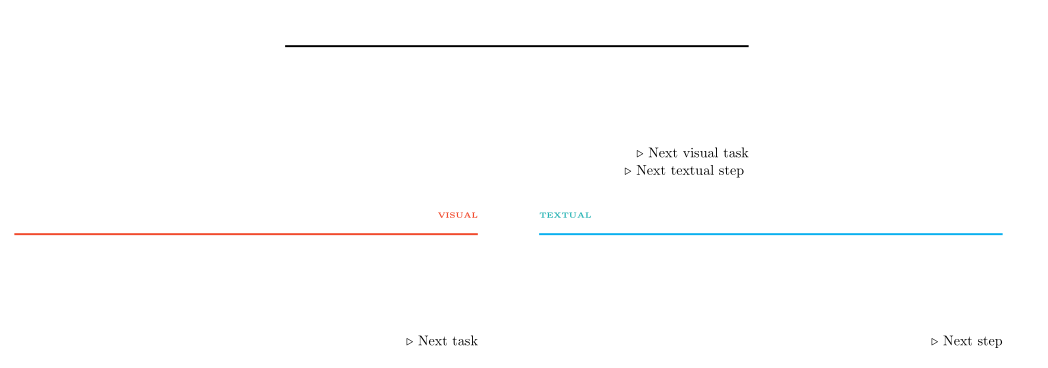
\includegraphics[width=1\textwidth]{pageExamples}
	\caption{Page Headers and Links} 
	\label{pageExamples} 
\end{figure}

At the end of each section, you'll find a \mbox{ $\triangleright$ {\texttt Next {\emph{label}}} } link. This is the link that will take you to the next
appropriate page. You are still welcome to go through the entire handbook page by page. In fact, we encourage it for our diagrams! We hope you can compare the
differences and similarities between the two sytanxes. But be warned - If what you're doing isn't matching what you see, you may be reading the wrong
instructions.

\pagebreak

If, however, you're finding that the screenshots we've taken aren't matching your screen and you ARE in the right place, please send us an email at
\href{mailto:contact@moflon.org}{contact@moflon.org} and let us know. They get outdated so fast! They just grow up, move on, start doing their own thing and
\ldots uh, wait a second. We're talking about pictures here.

Feel free to also contact us if you have any questions, concerns, or suggestions on ways we can improve.

\newpage

% Common instructions
\genHeader
\fancyfoot[RE]{ $\triangleright$ \hyperlink{installEA vis}{Next visual task} \\ $\triangleright$ \hyperlink{simpleDemo common}{Next textual step} }

\section{Install our plugin for Eclipse}
 
 \vspace{0.5cm}
 
\begin{itemize}
\item[$\blacktriangleright$] Download and install Eclipse for Modelling ``Eclipse Modeling Tools (includes incubating components)''\footnote{Please note that you \emph{have to} install \emph{Eclipse Modeling Tools}, from the Juno download packages, or nothing will work.  Do not choose a different Eclipse package!  Although different versions might work, eMoflon is currently tested for Eclipse Juno and Java 1.7.} from \url{http://www.eclipse.org/downloads/packages/release/juno/sr2} (Fig.~\ref{fig_downloadModelingPackage}).

\vspace{1.5cm}

\begin{figure}[htbp]
	\centering
  	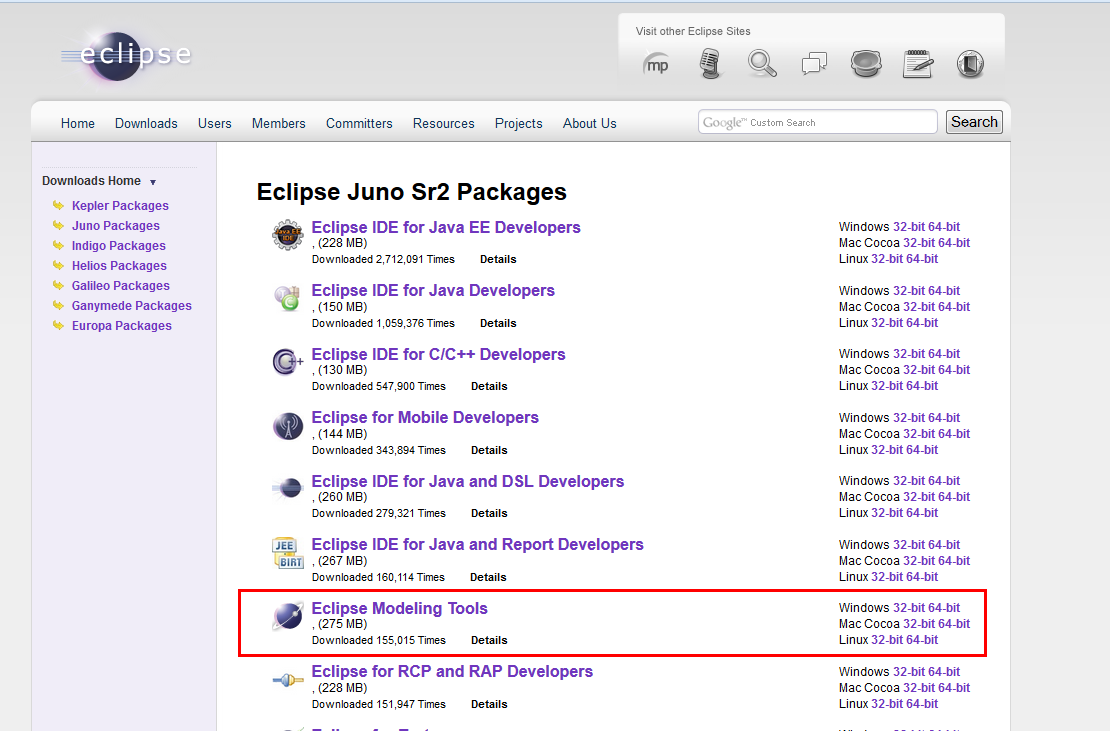
\includegraphics[width=0.86\textwidth]{eclipse_modelingTools}
	\caption{Download Eclipse Modeling Tools.}
	\label{fig_downloadModelingPackage}
\end{figure}

\vspace{1cm}

\item[$\blacktriangleright$] Install our Eclipse Plugin from the following update site\footnote{For a detailed tutorial on how to install Eclipse and Eclipse Plugins please refer to \url{http://www.vogella.de/articles/Eclipse/article.html}} 
\footnote{Please note: Calculating requirements and dependencies when installing the plugin might take quite a while depending on your internet connection.}:
\url{http://www.moflon.org/fileadmin/download/moflon-ide/eclipse-plugin/update-site2}

\end{itemize}


% Visual instructions; install EA
% -----------------------------------------------------------------------------------------------------------------------------------
% -------- VISUAL -------------------------------------------------------------------------------------------------------------------
\newpage

\section{Install our extension for Enterprise Architect}

\input{../02_EAExtension/visSources/page01}

\input{../02_EAExtension/texSources/page01}

\newpage
\genHeader

\section{Get a simple demo running}


\begin{itemize}
\hypertarget{simpleDemo common}{} 
\item[$\blacktriangleright$] Open Eclipse to a clean, fresh workspace. Go to ``Window/Open Perspective/Other\ldots''
\footnote{A path given as ``foo/bar'' indicates how to navigate in a series of menus and toolbars. Items you can open or click on-screen will be given in a
\texttt{different} font, new defintions or concepts will be \emph{italiziced}, and any data you're required to enter will be give as 'foo.'} and choose
\texttt{eMoflon}~(Fig.~\ref{fig_eclipse}).

\begin{figure}[htbp]
	\centering
  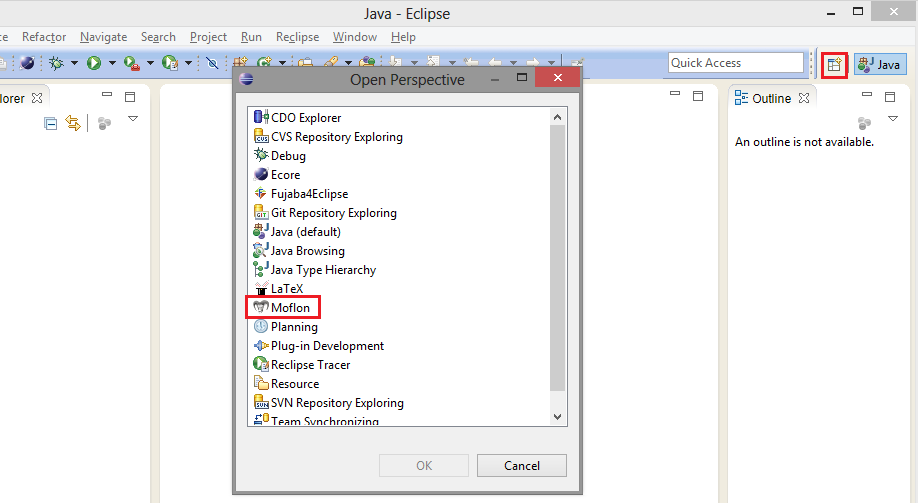
\includegraphics[width=\textwidth]{eclipse_firststart}
	\caption{Choose the eMoflon perspective {\bf update}}
	\label{fig_eclipse}
\end{figure} 

\item[$\blacktriangleright$] At either the far right, or center of the toolbar, a new action set should have appeared. Choose ``New Metamodel''
(Fig.~\ref{fig_eclipseNewMetamodelButton}).

\begin{figure}[htbp]
	\centering
  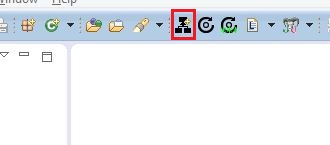
\includegraphics[width= 0.8\textwidth]{eclipse_newMetamodelButton}
	\caption{Invoke the ``New Metamodel'' wizard}
	\label{fig_eclipseNewMetamodelButton}
\end{figure}

%\nxtPage{\thepage}

\item[$\blacktriangleright$] A new dialog box should appear. This is the place where you officially decide which eMoflon syntax you'd like to use
(Fig.~\ref{fig_chooseSyntax}). With the visual syntax, you'll be using Eclipse alongside EA. You'll use EA to specify several kinds of diagrams, export, and
refresh your workspace in Eclipse. With the textual syntax (MOSL\footnote{eMoflon Specification Language}), you'll be working entirely within the Eclipse IDE.
No matter which syntax you choose however, give your project a name and make sure the \texttt{Add Demo Specification} button is selected. This will create all the
files and tests required to ensure you've set up eMoflon correctly.

\vspace{1cm}

\begin{figure}[htbp]
	\centering
  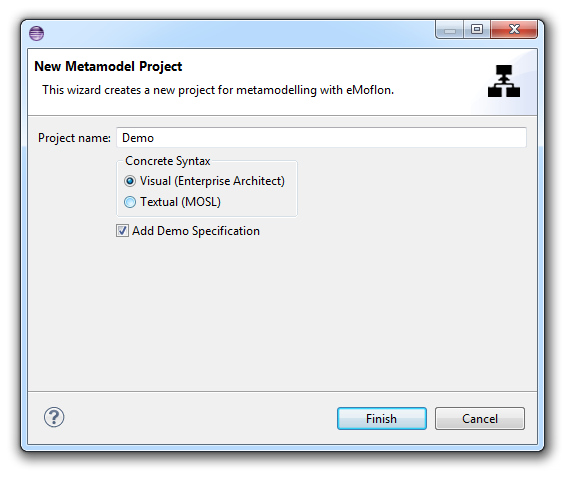
\includegraphics[width=0.9\textwidth]{eclipse_newMetamodelDialog}
	\caption{Choose your syntax}
	\label{fig_chooseSyntax}
\end{figure} 

\vspace{1cm}

% Edit me in the morning? I don't like the way this is written..
\item[$\blacktriangleright$]  Another new action on the toolbar is a button with an ``L'' on it (Fig.~\ref{fig_logger}). A log file is written everytime
you save your file, and appears in the eMoflon console window found below the main editor. This log contains important information for us if anything goes
wrong! You can silence certain loggers, set the level of loggers, and configure other settings\footnote{If you're not sure how to do this, check out a short
Log4j tutorial at \href{http://logging.apache.org/log4j/1.2/manual.html}{http://logging.apache.org/log4j/1.2/manual.html}} by clicking on this button and
modifying the \texttt{log4jConfig.properties} file.

\newpage
\vspace*{3cm}
\begin{figure}[htbp]
	\centering
  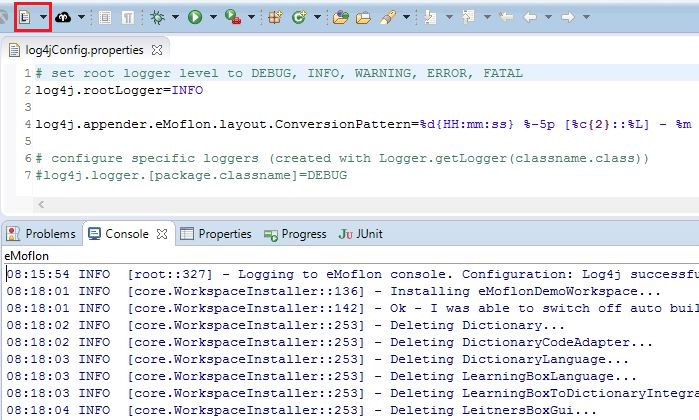
\includegraphics[width=0.9\textwidth]{eclipse_logger}
	\caption{The eMoflon logger}
	\label{fig_logger}
\end{figure} 
\end{itemize}

\fancyfoot[R]{ $\triangleright$ \hyperlink{simpleDemo vis}{Next [visual]\hspace{0.2cm}} \\ $\triangleright$ \hyperlink{simpleDemo tex}{Next [textual]}}

\clearpage
\visHeader

\subsection{A first look at Enterprise Architect}

\begin{itemize}
\FloatBarrier
\hypertarget{simpleDemo vis}{}
\item[$\blacktriangleright$] Can you locate the new \texttt{Demo.eap} file in your package explorer? This is the EA project file you'll be
modelling in. Don't worry any other folders at the moment - all problems will be resolved by the end of this section.

In the meantime, do not rename, move, or delete anything.

\item[$\blacktriangleright$] Double-click \texttt{Demo.eap} to start EA, and choose \texttt{Ultimate} when starting EA for the first time.

\item[$\blacktriangleright$] In EA, navigate to ``Extensions/MOFLON::Ecore Addin/Export\- all\- to\- Workspace'' (Fig.~\ref{fig:ea}). 

\begin{figure}[htbp]
	\centering
  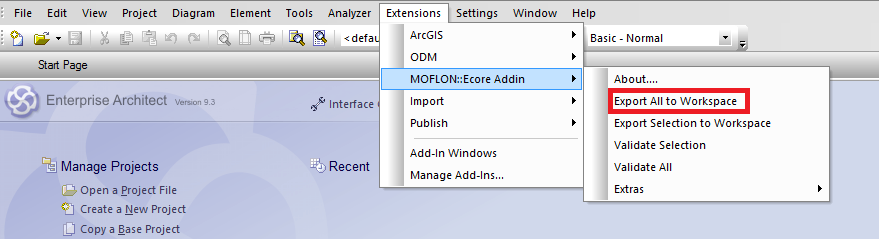
\includegraphics[width=0.9\textwidth]{ea_firststart}
	\caption{Export from EA} 
	\label{fig:ea} 
\end{figure}

\item[$\blacktriangleright$] Please note that this submenu is limited, and does not provide access to all eMoflon functionality. You can activate eMoflon's full
control panel window by going to ``Extensions/Add-In Windows'' (Fig.~\ref{fig:controlPanel}). To export from here, click \texttt{All} in the ``Export'' section.

\begin{figure}[htbp]
	\centering
  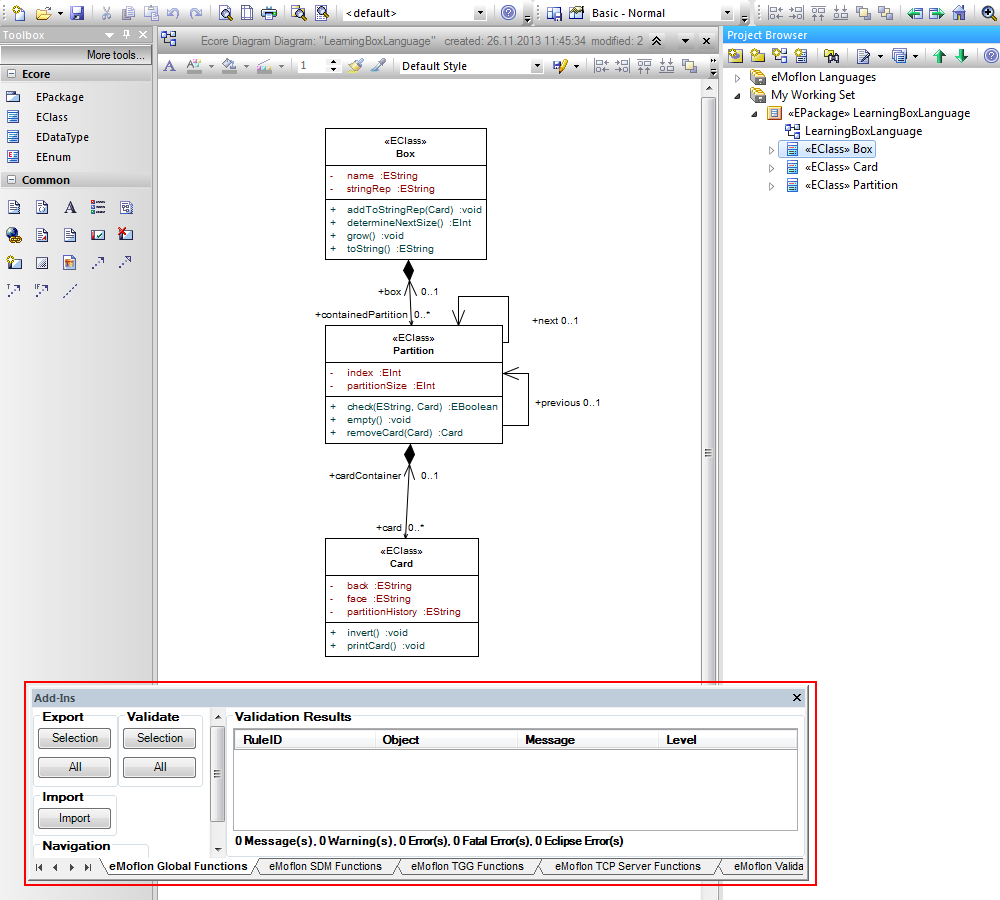
\includegraphics[width=0.9\textwidth]{ea_controlPanel}
	\caption{eMoflon's control panel} 
	\label{fig:controlPanel} 
\end{figure}

\item[$\blacktriangleright$] Now try exploring the EA project browser! Try to navigate to the packages, classes, and diagrams. Don't worry if you don't
understand that much - we'll get to explaining everything in a moment. Just make sure not to change anything!

%\nxtPage{\thepage}
\newpage

\item[$\blacktriangleright$] Switch back to Eclipse, choose your metamodel project, and press F5 to refresh. A new folder should appear, and your errors should
disappear after a few seconds. Since you've chosen to use our visual syntax, there isn't much to look at here. The export from EA places all required files in a
hidden folder(.temp) in the project, and refreshing triggers a build process that invokes our code generator automatically. 

\item[$\blacktriangleright$] You should be able to monitor the progress with the green bar in the lower right corner (Fig.~\ref{fig_eclipseBuild}). Pressing the
symbol opens a monitor view that gives more details of the build process. You don't need to worry about any of these details, just remember to refresh your
Eclipse workspace after an export.

\fancyfoot[OR]{$\triangleright$ \hyperlink{validate common}{Next}}

\begin{figure}[htbp]
	\centering
  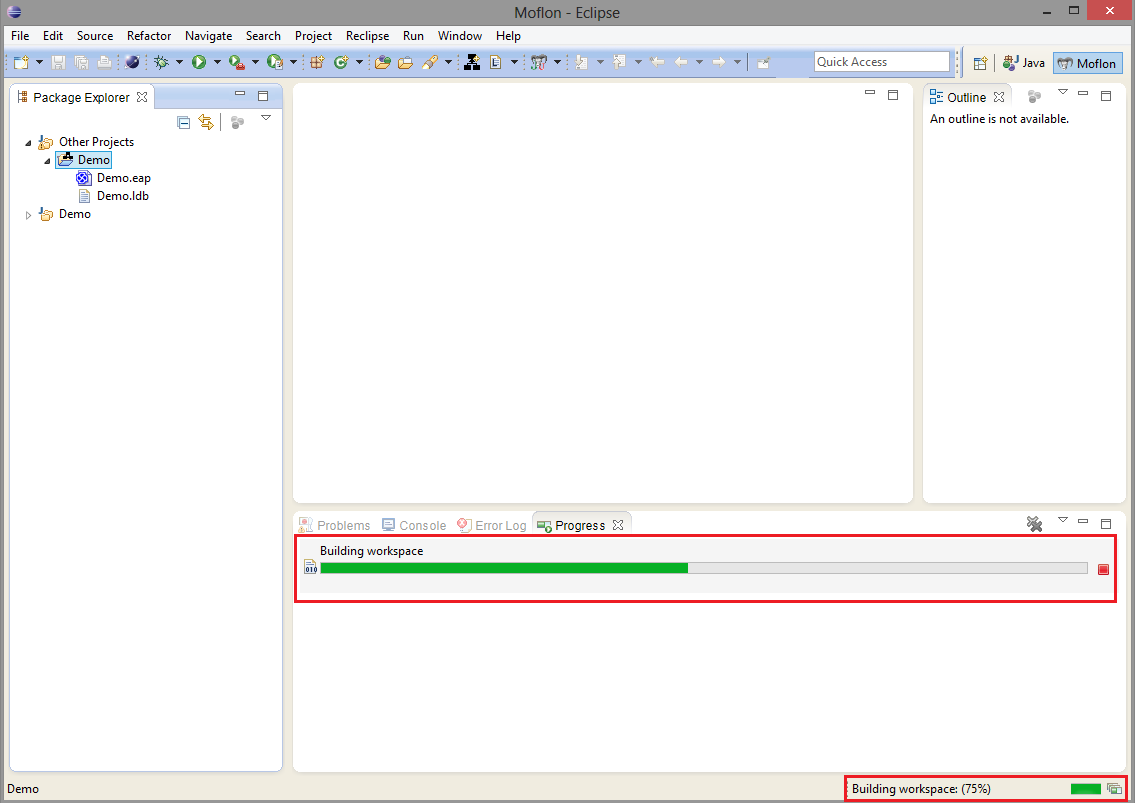
\includegraphics[width=0.9\textwidth]{eclipse_building}
	\caption{Eclipse workspace when using visual syntax} 
	\label{fig_eclipseBuild} 
\end{figure}

\item[$\blacktriangleright$] If you're ever worried about forgetting to refresh your workspace, or if you just don't want to bother with having to do this,
Eclipse does offer an option to do it for you automatically. To activate this, Go to ``Window/Preferences/General/Workspace" and select \texttt{refresh on
access}.

\end{itemize}

\newpage
\texHeader
% \fancyfoot[R]{$\triangleright$ \hyperlink{validate common}{Next}}

\subsection{A first look at MOSL}

\begin{itemize}
\FloatBarrier
\hypertarget{simpleDemo tex}{} 
\item[$\blacktriangleright$] You should immediately have 3 folders available in your project explorer - Your metamodel project,
\texttt{DoubleLinkedListLanguage}, and \\ \texttt{texDemoTestSuite}. Initially, you'll see a red exclamation mark indicating there are errors, but once you give
Eclipse a few seconds to refresh, all problems should be solved.

\item[$\blacktriangleright$] That's it! You're all set up! But, while you're here, feel free to explore the ``Demo'' folder. It has the basic code that implements
this demo, and we recommend you take a brief look to get a feel for the the general syntax.

In the meantime, please do not rename, move, or delete anything.
\end{itemize}


\newpage
\genHeader
\fancyfoot[R]{ $\triangleright$ \hyperlink{projectStructure vis}{Next visual task} \\ $\triangleright$ \hyperlink{projectStructure tex}{Next textual step} }

\section{Validate your installation with JUnit}

\begin{itemize}

\item[$\blacktriangleright$] In\hypertarget{validate common}{} the eclipse workspace, choose ``Working Sets'' as your top level element in the package explorer (Fig.~\ref{fig_topLevel}). We work with many working sets, and use them to structure the workspace in Eclipse.

\begin{figure}[htbp]
	\centering
  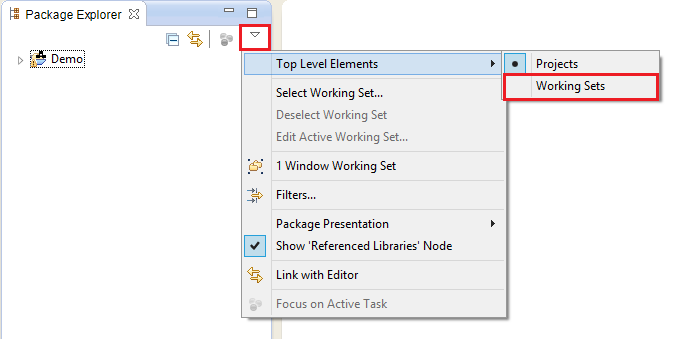
\includegraphics[width=1\textwidth]{eclipse_workingsets}
	\caption{Top Level Elements in Eclipse}
	\label{fig_topLevel}
\end{figure}

\item[$\blacktriangleright$] The files have now been restructured and sorted into three nodes. The organization for these nodes will be explained in a moment but for now, check out ``Other Projects/DemoTestSuite.'' This is the testing unit imported with the demo files to make sure everything was installed and set up correctly. Right click on the Project to bring up the context menu and press ``Run As/JUnit Test.'' If anything goes wrong, try refereshing by choosing folders and pressing  \texttt{F5}, or right-clicking and selecting ``Refresh.''

\vspace{0.5cm}

\begin{figure}[htbp]
	\centering
  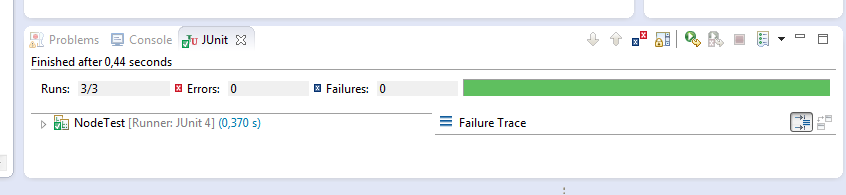
\includegraphics[width=1\textwidth]{eclipse_passedJUnitTest}
	\caption{All's well that ends well\ldots}
	\label{fig_passedTest}
\end{figure}

\vspace{0.5cm}

Congratulations!  If you see a green bar  (Fig.~\ref{fig_passedTest}), then everything has been set up correctly and you are now ready to start metamodelling!

\end{itemize}

\newpage
\section{Project setup}

% No new page; first page call under this section. see ProjectStructureSrc . 
\genHeader

\subsection{Your Enterprise Architect Workspace}

Now\hypertarget{projectStructure vis}{} that everything is installed and setup properly, let's take a closer look at the different workspaces and our workflow.
Before we continue, please make a few slight adjustments to Enterprise Architect (EA) so you can easily compare your current workspace to our screenshots.
These settings are advisable but you are, of course, free to choose your own colour schema.

\begin{stepbystep}

\item  Select \menuPath{Tools \menuSep Options \menuSep Themes} in EA, and set Diagram Theme to \texttt{Enterprise Architect 10}.

\item  Next, proceed to \menuPath{Gradients and Background} and set \menuPath{Gradient} and \menuPath{Fill} to \entity{White} (\Cref{ea:paperAndElementFill}). 

\begin{figure}[htbp]
    \centering
    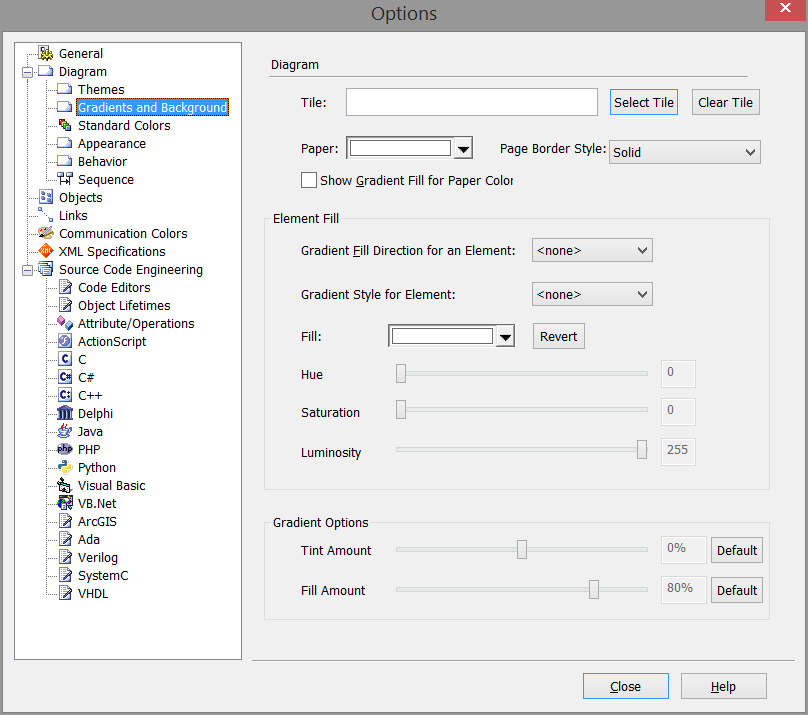
\includegraphics[width=0.8\textwidth]{standardPaperAndFill}
    \caption{Suggested paper background and element fill}
    \label{ea:paperAndElementFill}
\end{figure}

\item  In the \menuPath{Standard Colors} tab, and set your colours to reflect \Cref{ea:standardColoursEA}.

\begin{figure}[htbp]
  \centering
  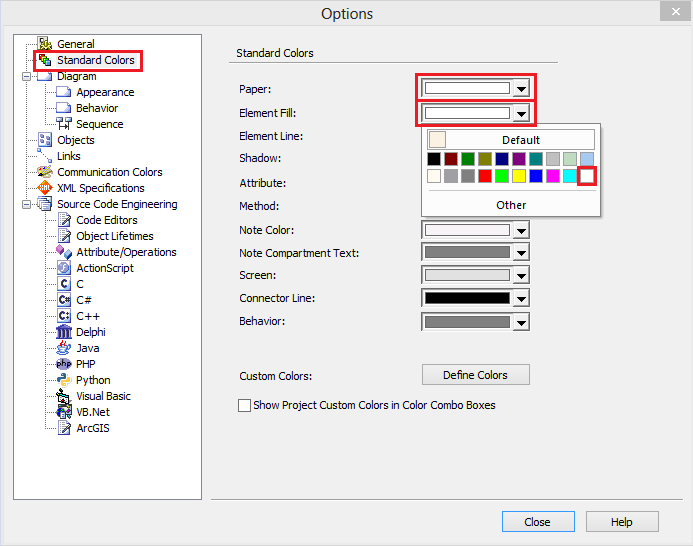
\includegraphics[width=0.8\textwidth]{standardColours}
  \caption{Our choice of standard colours for diagrams in EA}
  \label{ea:standardColoursEA}
\end{figure}

\vspace{0.5cm}

\item 
In the same dialogue, go to \menuPath{Diagram \menuSep Appearance} and reflect the settings in \Cref{ea:standardAppearanceEA}.
Again, this is just a suggestion and not mandatory.

\item 
Last but not least open the \menuPath{Code Engineering} toolbar (\Cref{ea:standardSCEEA1}) and choose \entity{Ecore} as the default language (\Cref{ea:standardSCEEA2}).
\textbf{This setting is mandatory, and very important.}
\end{stepbystep}

\begin{figure}[htbp]
  \centering
  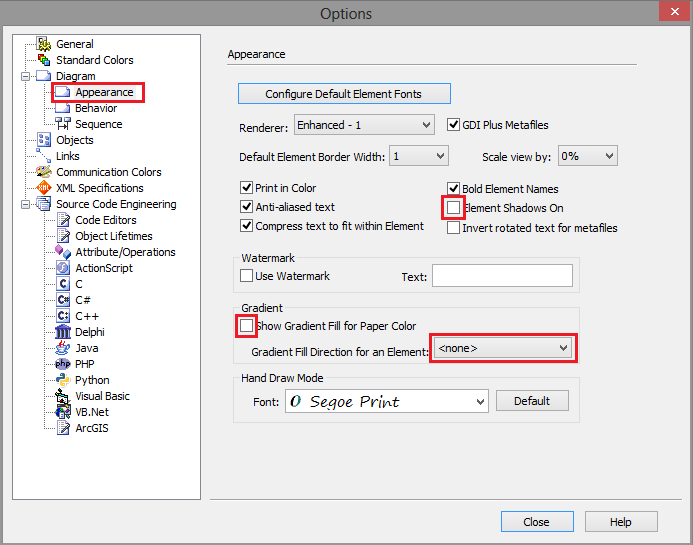
\includegraphics[width=0.8\textwidth]{standardAppearance}
  \caption{Our choice of the standard appearance for model elements}
  \label{ea:standardAppearanceEA}
\end{figure}

\begin{figure}[htbp]
    \centering
    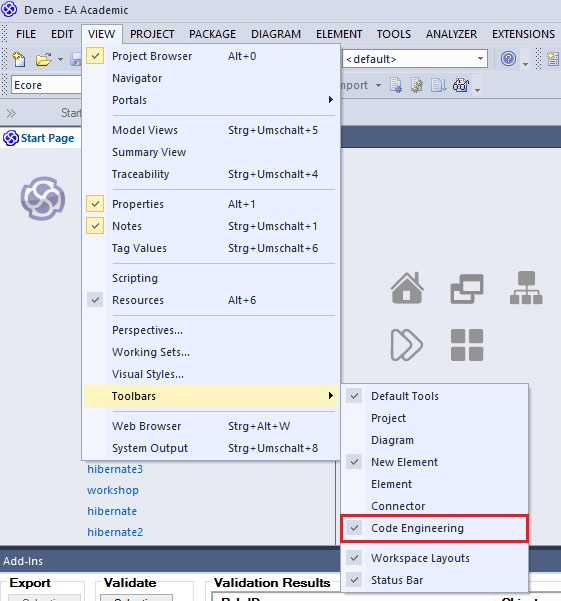
\includegraphics[width=0.8\textwidth]{standardCodeEngineering1}
    \caption{Open the \menuPath{Code Engineering} toolbar}
    \label{ea:standardSCEEA1}
 \end{figure}

\begin{figure}[htbp]
    \centering
    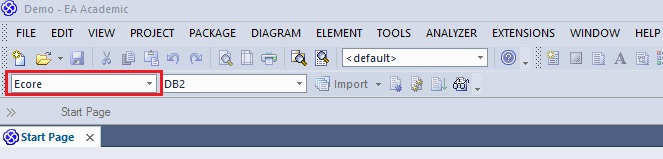
\includegraphics[width=0.8\textwidth]{standardCodeEngineering2}
    \caption{Make sure you set the standard language to \entity{Ecore}}
    \label{ea:standardSCEEA2}
 \end{figure}
 
\clearpage

In your EA \enquote{workspace} (actually referred to as an \emph{EA project}), take a careful look at the project browser:
The root node \texttt{Demo} is called a \emph{model} in EA lingo, and is used as a container to group a set of related \emph{packages}.
In our case, \texttt{Demo} contains a single package \texttt{org.moflon.demo.doublelinkedlist}.
An EA project however, can consist of numerous models that in turn, group numerous packages.

Now switch back to your Eclipse workspace and note the two nodes named \texttt{Specifications} and \texttt{org.moflon.demo} (\Cref{eclipse:eclipsePS}).

\begin{figure}[htbp]
    \centering
    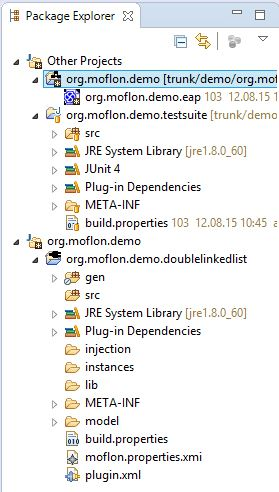
\includegraphics[width=0.4\textwidth]{eclipse_visPackageExplorer}
    \caption{Project structure}
    \label{eclipse:eclipsePS}
 \end{figure}

These nodes, used to group related \emph{Eclipse projects} in an Eclipse workspace, are called \emph{working sets}. The working set
\texttt{Spe\-ci\-fi\-ca\-tions} contains all \emph{metamodel projects} in a  workspace. Your metamodel project contains a single EAP (EA project) file and is
used to communicate with EA and initiate code generation by simply pressing \texttt{F5} or choosing \texttt{Refresh} from the context menu. In our case,
\texttt{Specifications} should contain a single metamodel project \texttt{org.moflon.demo} containing our EA project file \texttt{org.moflon.demo.eap}.
 
\Cref{fig:fromEAtoEclipse} depicts how the Eclipse working set \texttt{org.moflon.demo} and its contents were generated from the EA model \texttt{org.moflon.demo}. Every model
in EA is mapped to a working set in Eclipse with the same name. From every package in the EA model, an Eclipse project is generated, also with the same name.
%\LK{Fix names and screenshot (does not match previous figure)}

\begin{figure}[htbp]
    \centering
  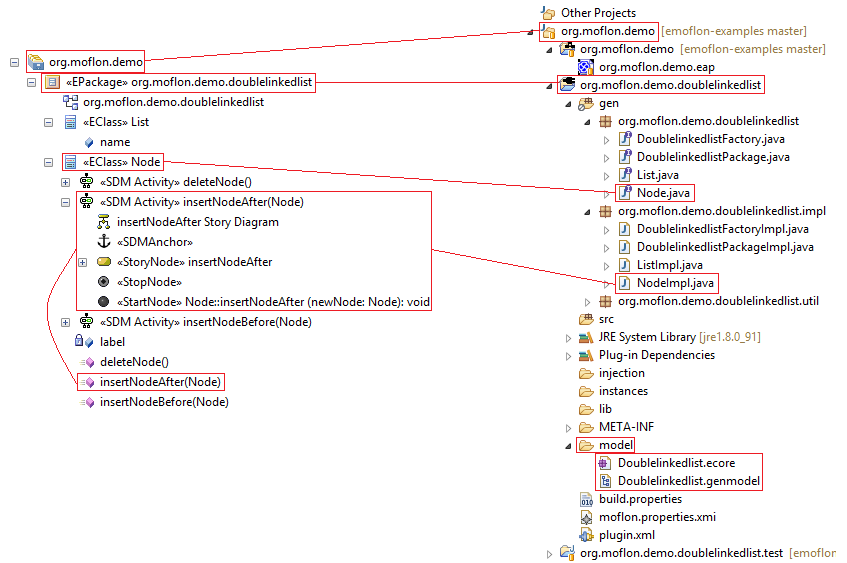
\includegraphics[width=\textwidth]{fromEAToEclipse}
    \caption{Mapping between artefacts in EA and Eclipse}
    \label{fig:fromEAtoEclipse}
\end{figure}

These projects, however, are of a different nature than, for example, metamodel projects or normal Java projects.
These are called \emph{repository projects}.
A \newconcept{nature} is Eclipse lingo for \enquote{project type} and is visually indicated by a corresponding nature icon on the project folder.
Our metamodel projects sport a neat little class diagram symbol.
Repository projects are generated automatically with a certain project structure according to our conventions.

The \entity{model} subfolder in the Eclipse package explorer is probably the most important as it contains the \newconcept{Ecore model} for the project. Ecore is a metamodeling language that provides building blocks such as \newconcept{classes} and \newconcept{references} for defining the static structure (concepts and relations between concepts) of a system.
This folder also contains a \newconcept{genmodel}, the second model required by the Eclipse Modeling Framework (EMF) to generate Java code.

Looking back to \Cref{fig:fromEAtoEclipse}, realize that it also depicts how the class \entity{Node} in the EA model is mapped to the Java interface \entity{Node}.
Double-click \entity{Node.java} and take a look at the methods declared in the interface. These correspond directly to the methods declared in the modeled \entity{Node} class.

As indicated by the source folders \entity{src}, \entity{injection}, and \entity{gen}, we advocate a clean separation of hand-written (should be placed in \entity{src} and \entity{injection}) and generated code (automatically in \texttt{gen}).
As we shall see later in the handbook, hand-written code can be
integrated in generated classes via \emph{injections}.
This is sometimes necessary for small helper functions.

Have you noticed the methods of the \entity{Node} class in our EA model? 
Now hold on tight---each method can be \newconcept{modeled} completely in EA and the corresponding implementation in Java is generated automatically and placed in \texttt{NodeImpl.java}.
Just in case you didn't get it: The behavioural or dynamic aspects of a system can be completely modeled in an abstract, platform-/programming language--independent fashion using a blend of activity diagrams and a \enquote{graph pattern} language called \newconcept{Story~Driven~Modelling}~(SDM).
In our EA project, these \newconcept{Story Diagrams} or simply \emph{SDM}s, are placed in \newconcept{SDM Containers} named according to the method they implement.
For instance, \texttt{\guillemotleft{}SDM Activity\guillemotright{} insertNodeAfter SDM} for the method \texttt{in\-sert\-NodeAft\-er(Node)} as depicted in \Cref{fig:fromEAtoEclipse}.
We'll dedicate Part III of the handbook to understanding why SDMs are so  {\huge crazily} cool!

To recap all we've discussed, let's consider the complete workflow as depicted in \Cref{fig:Overview}. We started with a concise model in EA, simple and
independent of any platform specific details~(1).  Our EA model consists not only of static aspects modelled as a class diagram~(2), but also of dynamic aspects
modelled using SDM~(3).  After exporting the model and code generation~(4), we basically switch from \emph{modelling} to \emph{programming} in a specific
general purpose programming language (Java). On this lower \emph{level of abstraction}, we can flesh out the generated repository~(5) if necessary, and mix as
appropriate with hand-written code and libraries.  Our abstract specification of behaviour (methods) in SDM is translated to a series of method calls that form
the body of the corresponding Java method~(6).

\begin{figure}[htbp]
	\centering
  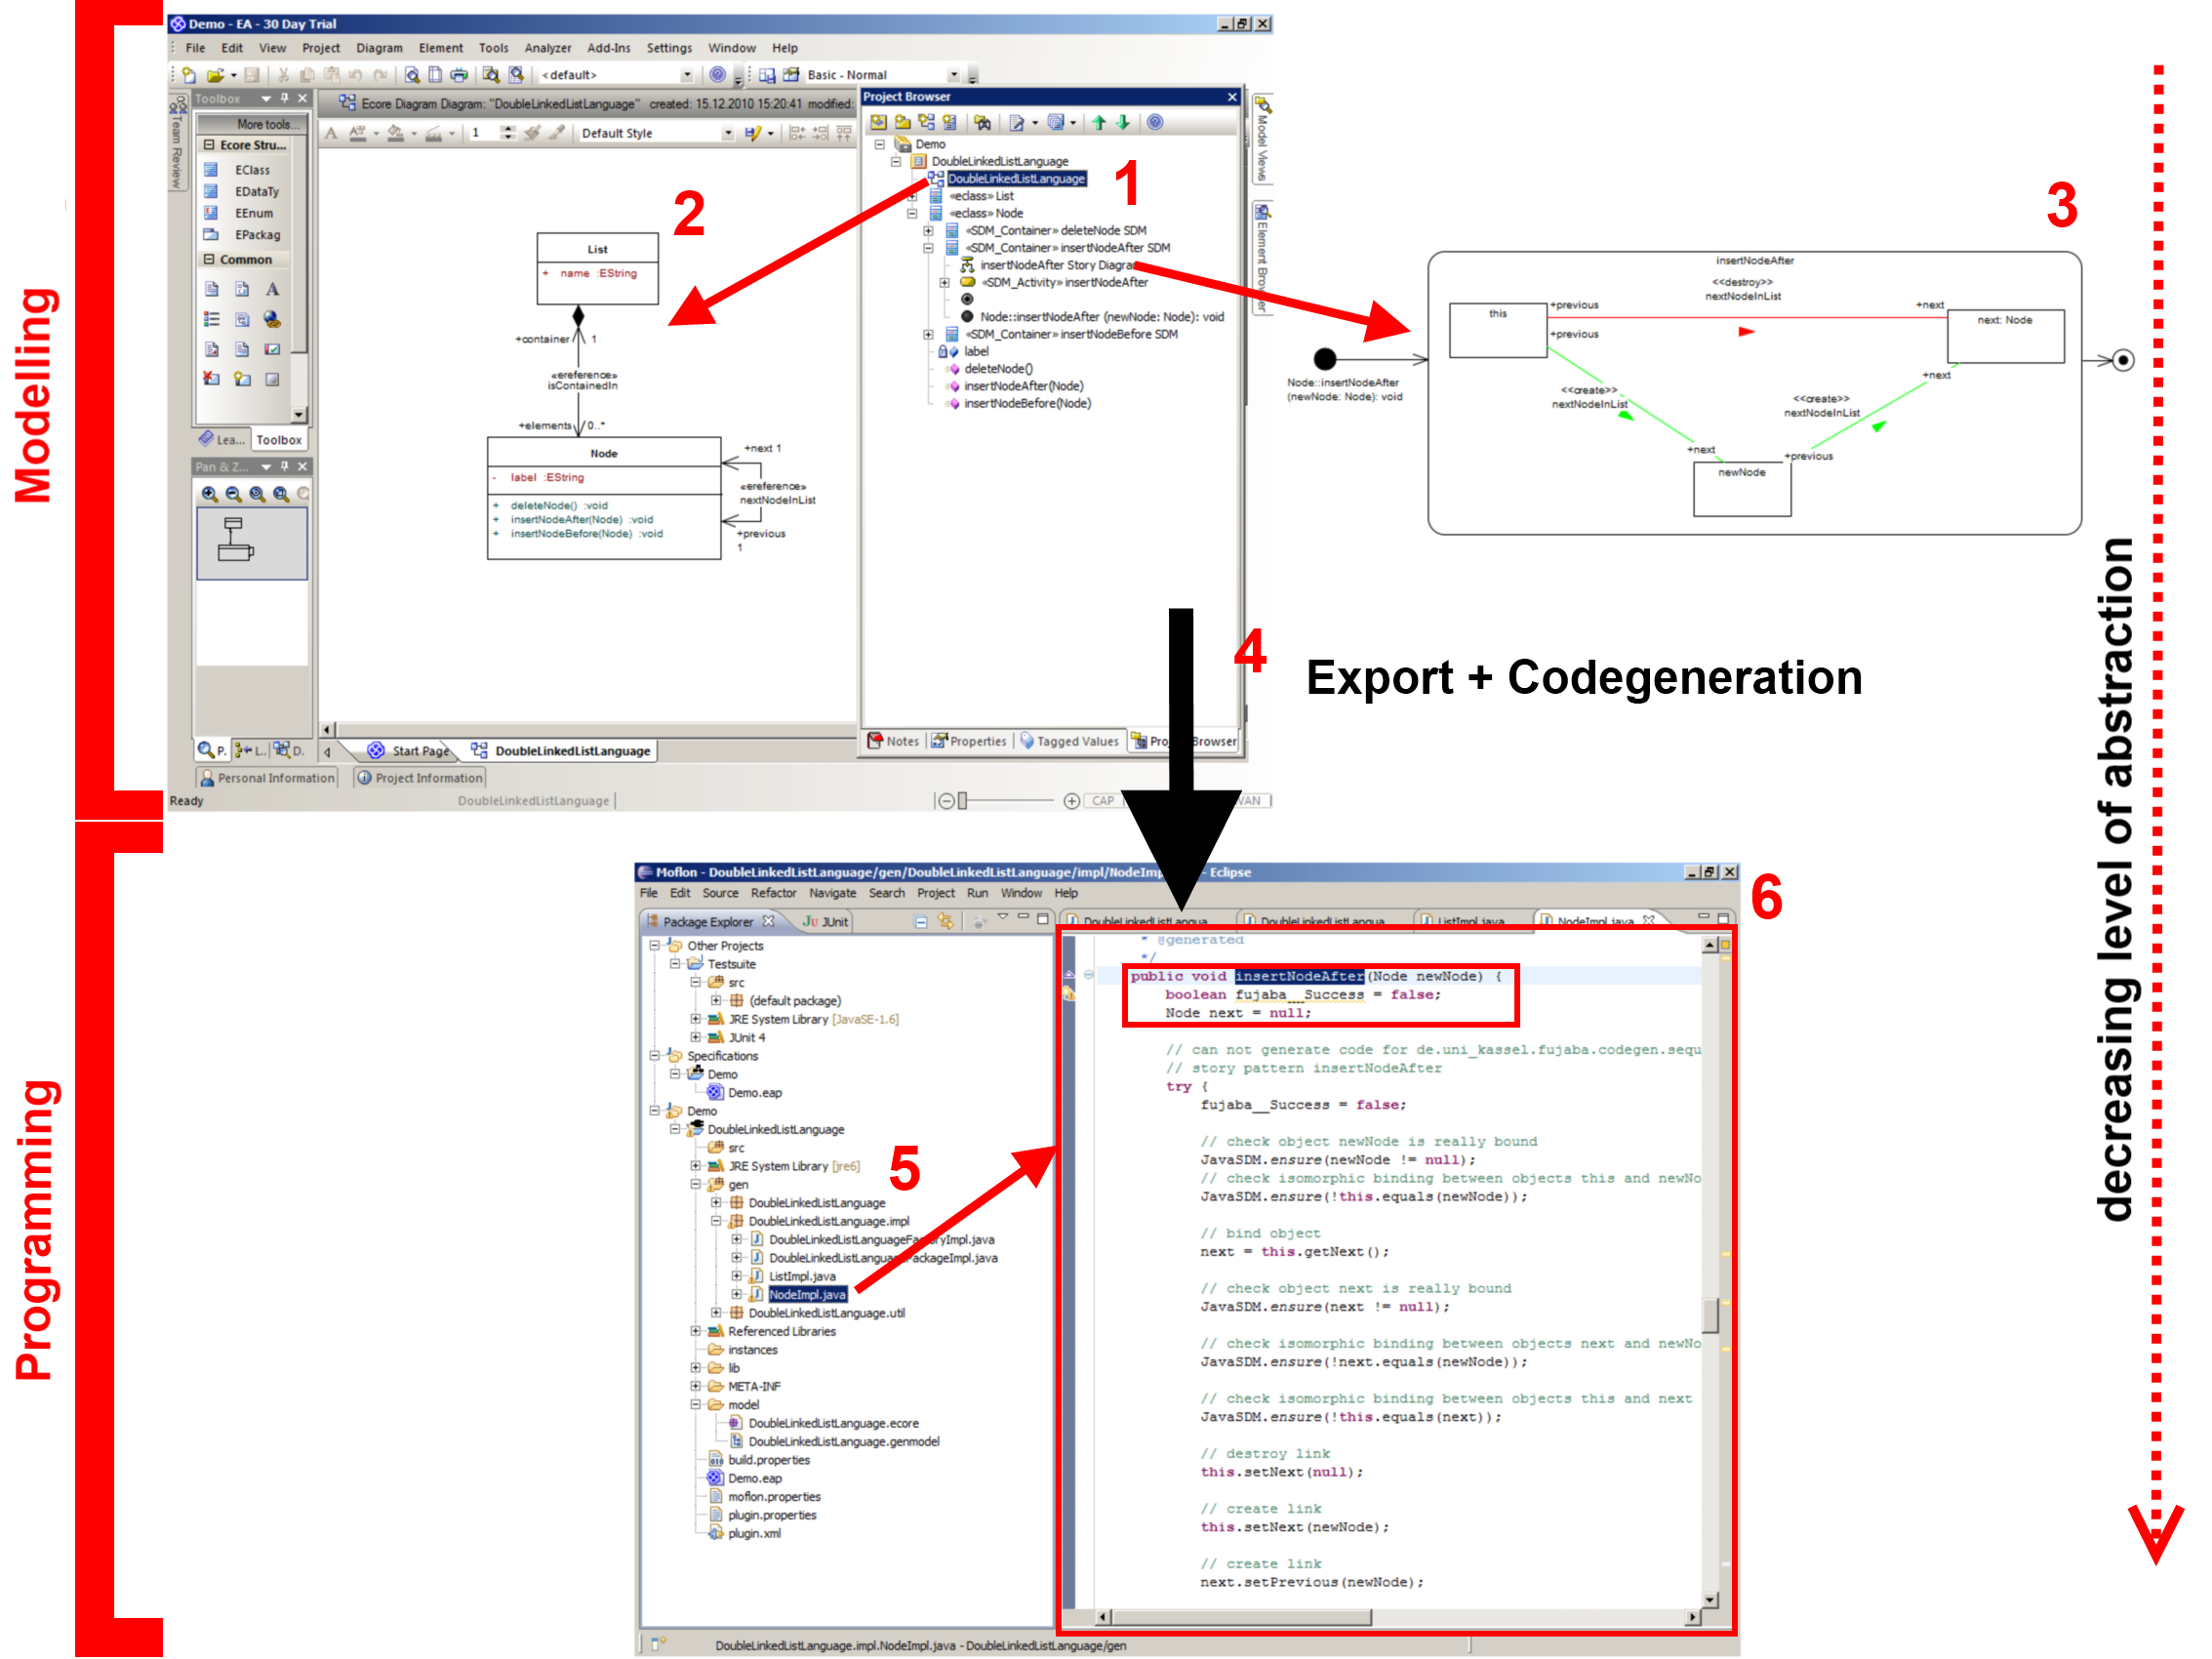
\includegraphics[width=1.1\textwidth]{tafelbild}
	\caption{Overview}
	\label{fig:Overview}
\end{figure}


\clearpage

\newpage
\genHeader
\hypertarget{codeGen common}{} 
\chapter{Generated code vs. hand-written code}

Now that you've worked through the specifics of your syntax, lets have a brief discussion on code generation.

The Ecore model is used to drive a code generator that maps the model to Java interfaces and classes. The generated Java code that represents the model is often
referred to as a repository. This is the reason why we refer to such projects as repository projects. A repository can be viewed as an adapter that enables
building and manipulating concrete instances of a specific model via a programming language such as Java. This is why we indicate repository projects using a
cute adapter/plug symbol on the project folder.

If you take a careful look at the code structure in \texttt{gen} (\Cref{eclipse:structureGen}), you'll find a \texttt{FooImpl.java} for every
\texttt{Foo.java}. Indeed, the subpackage \texttt{.impl} contains Java classes that implement the interfaces in the parent package. Although this might strike
you as unnecessary (why not merge interface and implementation for simple classes?), this consequent separation in interfaces and implementation allows for a
clean and relatively simple mapping of Ecore to Java, even in tricky cases such as multiple inheritance (allowed and very common in Ecore models). A further
package \texttt{.util} contains some auxiliary classes such as a factory for creating instances of the model.

 \begin{figure}[htbp]
  \centering
  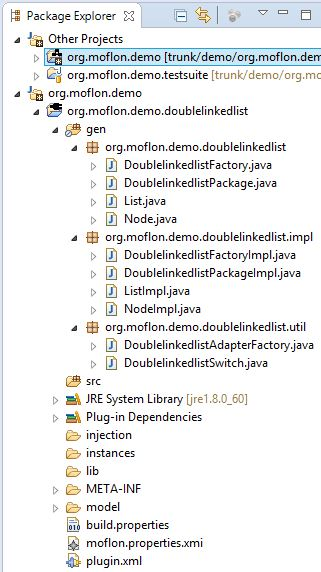
\includegraphics[width=0.4\textwidth]{../../org.moflon.doc.handbook.01_installation/5_codeGeneration/eclipse_structureGen}
  \caption{Package structure of generated code (\texttt{gen})}
  \label{eclipse:structureGen}
\end{figure}

If this is your first time of seeing generated code, you might be shocked at the sheer amount of classes and code generated from our relatively simple model.
You might be thinking: ``Hey -- if I did this by hand, I wouldn't need half of all this stuff!''  Well, you're right and you're wrong. The point is that an
automatic mapping to Java via a code generator scales quite well.

This means for simple, trivial examples (like our double linked list), it might be possible to come up with a leaner and simpler Java representation. For
complex, large models with lots of mean pitfalls however, this becomes a daunting task. The code generator provides you with years and \emph{years} of
experience of professional programmers who have thought up clever ways of handling multiple inheritance, an efficient event mechanism, reflection, consistency
between bidirectionally linked objects, and much more.

A point to note here is that the mapping to Java is obviously not unique. Indeed there exist different standards of how to map a modelling language to a
general purpose programming language such as Java. As previously mentioned, we use a mapping defined and implemented by the Eclipse Modelling Framework (EMF),
which tends to favour efficiency and simplicity over expressiveness and advanced features.

% 
{\bf \huge Part I:}
\vspace{0.7cm}
 
{\bf \Huge Installation and Setup }

\vspace{0.5cm}

This part provides a very simple example and a JUnit test to check the installation and configuration of eMoflon. It can be considered \emph{mandatory} if you
are new to eMoflon, but we recommend working through it anyway.

After working through this part, you should have an installed and tested eMoflon working for a trivial example. We also explain the general workflow, the
different workspaces involved, and general usage of both our visual and textual syntax.

{\small \texttt Approximate time: Just a few minutes \ldots}

\section{Getting Started}

% Welcome Summary
\genHeader \fancyfoot[ER]{  $\triangleright$ \hyperlink{installPlugin common}{Next} } {\small \texttt Approximate time: Just a few minutes \ldots}

This part provides a very simple example and a JUnit test to check the installation and configuration of eMoflon.

After working through this part, you should have an installed and tested eMoflon working for a trivial example. We also explain the general workflow, the
different workspaces involved and general useage of each syntax.

This part can be considered \emph{mandatory} if you are new to eMoflon, but we reccommend working through it anyway.

Here's how we've organized our handbooks; in this part we introduce the first black, red, and blue headers to separate the common, visual, and textual syntax
instructions (Fig~\ref{pageExamples}).

\begin{figure}[htbp] \centering
  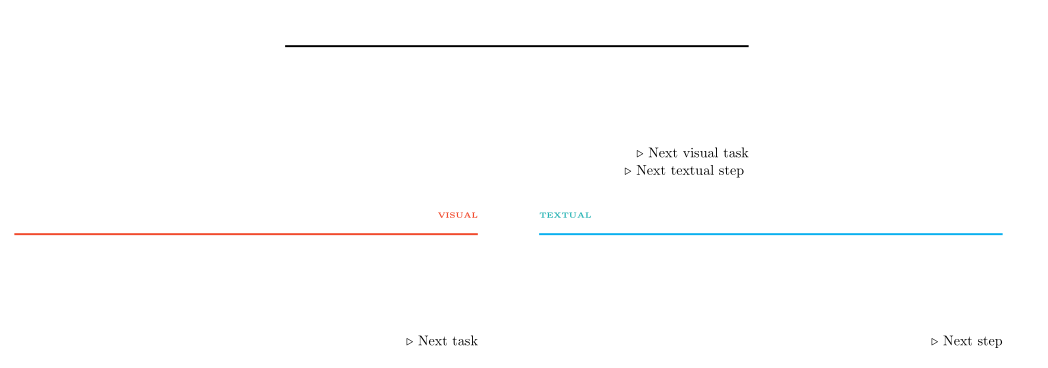
\includegraphics[width=1\textwidth]{pageExamples}
	\caption{Page Headers and Links} 
	\label{pageExamples} 
\end{figure}

At the end of each section, you'll find a \mbox{ $\triangleright$ {\texttt Next {\emph{label}}} } link. This is the link that will take you to the next
appropriate page. You are still welcome to go through the entire handbook page by page. In fact, we encourage it for our diagrams! We hope you can compare the
differences and similarities between the two sytanxes. But be warned - If what you're doing isn't matching what you see, you may be reading the wrong
instructions.

\pagebreak

If, however, you're finding that the screenshots we've taken aren't matching your screen and you ARE in the right place, please send us an email at
\href{mailto:contact@moflon.org}{contact@moflon.org} and let us know. They get outdated so fast! They just grow up, move on, start doing their own thing and
\ldots uh, wait a second. We're talking about pictures here.

Feel free to also contact us if you have any questions, concerns, or suggestions on ways we can improve.

\newpage

% Common instructions
\genHeader
\fancyfoot[RE]{ $\triangleright$ \hyperlink{installEA vis}{Next visual task} \\ $\triangleright$ \hyperlink{simpleDemo common}{Next textual step} }

\section{Install our plugin for Eclipse}
 
 \vspace{0.5cm}
 
\begin{itemize}
\item[$\blacktriangleright$] Download and install Eclipse for Modelling ``Eclipse Modeling Tools (includes incubating components)''\footnote{Please note that you \emph{have to} install \emph{Eclipse Modeling Tools}, from the Juno download packages, or nothing will work.  Do not choose a different Eclipse package!  Although different versions might work, eMoflon is currently tested for Eclipse Juno and Java 1.7.} from \url{http://www.eclipse.org/downloads/packages/release/juno/sr2} (Fig.~\ref{fig_downloadModelingPackage}).

\vspace{1.5cm}

\begin{figure}[htbp]
	\centering
  	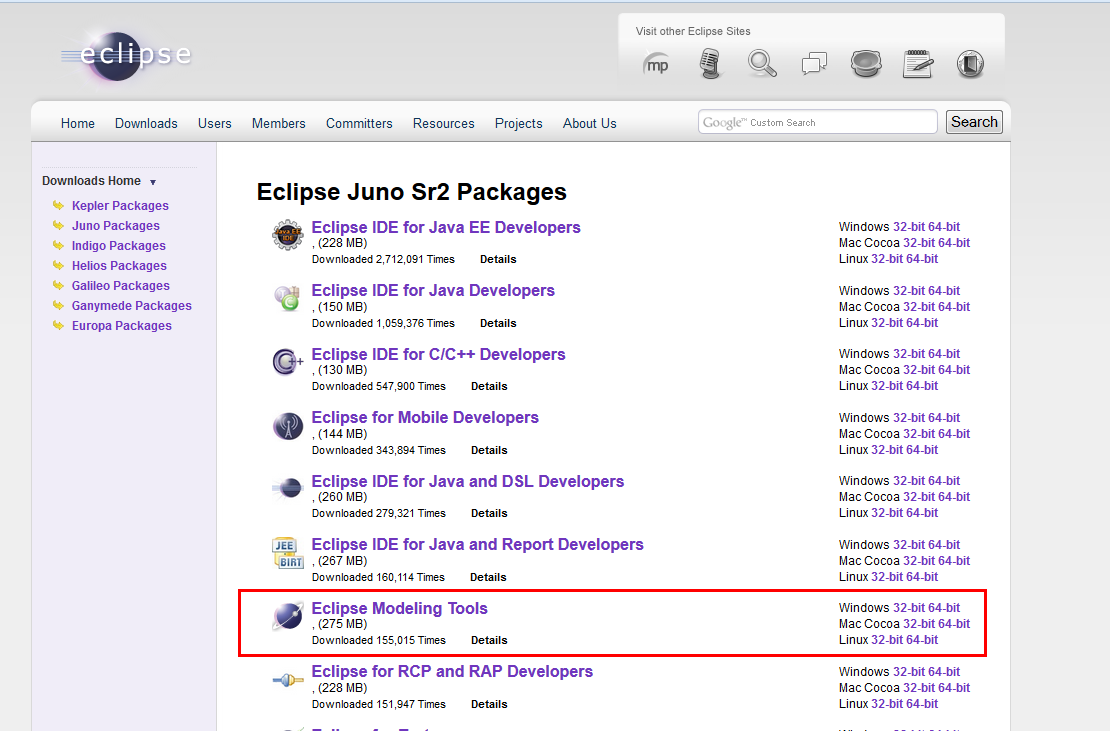
\includegraphics[width=0.86\textwidth]{eclipse_modelingTools}
	\caption{Download Eclipse Modeling Tools.}
	\label{fig_downloadModelingPackage}
\end{figure}

\vspace{1cm}

\item[$\blacktriangleright$] Install our Eclipse Plugin from the following update site\footnote{For a detailed tutorial on how to install Eclipse and Eclipse Plugins please refer to \url{http://www.vogella.de/articles/Eclipse/article.html}} 
\footnote{Please note: Calculating requirements and dependencies when installing the plugin might take quite a while depending on your internet connection.}:
\url{http://www.moflon.org/fileadmin/download/moflon-ide/eclipse-plugin/update-site2}

\end{itemize}


% Visual instructions; install EA
% -----------------------------------------------------------------------------------------------------------------------------------
% -------- VISUAL -------------------------------------------------------------------------------------------------------------------
\newpage

\section{Install our extension for Enterprise Architect}

\input{../02_EAExtension/visSources/page01}

\input{../02_EAExtension/texSources/page01}

\newpage
\genHeader

\section{Get a simple demo running}


\begin{itemize}
\hypertarget{simpleDemo common}{} 
\item[$\blacktriangleright$] Open Eclipse to a clean, fresh workspace. Go to ``Window/Open Perspective/Other\ldots''
\footnote{A path given as ``foo/bar'' indicates how to navigate in a series of menus and toolbars. Items you can open or click on-screen will be given in a
\texttt{different} font, new defintions or concepts will be \emph{italiziced}, and any data you're required to enter will be give as 'foo.'} and choose
\texttt{eMoflon}~(Fig.~\ref{fig_eclipse}).

\begin{figure}[htbp]
	\centering
  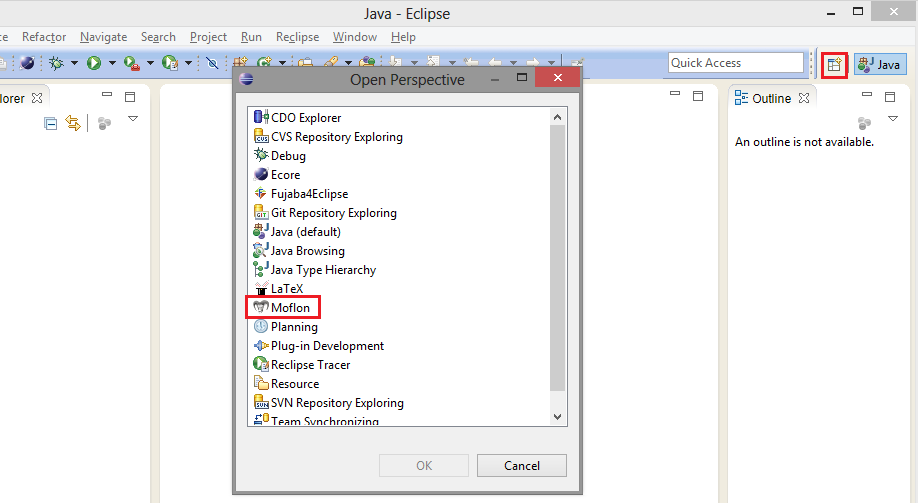
\includegraphics[width=\textwidth]{eclipse_firststart}
	\caption{Choose the eMoflon perspective {\bf update}}
	\label{fig_eclipse}
\end{figure} 

\item[$\blacktriangleright$] At either the far right, or center of the toolbar, a new action set should have appeared. Choose ``New Metamodel''
(Fig.~\ref{fig_eclipseNewMetamodelButton}).

\begin{figure}[htbp]
	\centering
  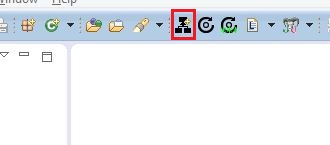
\includegraphics[width= 0.8\textwidth]{eclipse_newMetamodelButton}
	\caption{Invoke the ``New Metamodel'' wizard}
	\label{fig_eclipseNewMetamodelButton}
\end{figure}

%\nxtPage{\thepage}

\item[$\blacktriangleright$] A new dialog box should appear. This is the place where you officially decide which eMoflon syntax you'd like to use
(Fig.~\ref{fig_chooseSyntax}). With the visual syntax, you'll be using Eclipse alongside EA. You'll use EA to specify several kinds of diagrams, export, and
refresh your workspace in Eclipse. With the textual syntax (MOSL\footnote{eMoflon Specification Language}), you'll be working entirely within the Eclipse IDE.
No matter which syntax you choose however, give your project a name and make sure the \texttt{Add Demo Specification} button is selected. This will create all the
files and tests required to ensure you've set up eMoflon correctly.

\vspace{1cm}

\begin{figure}[htbp]
	\centering
  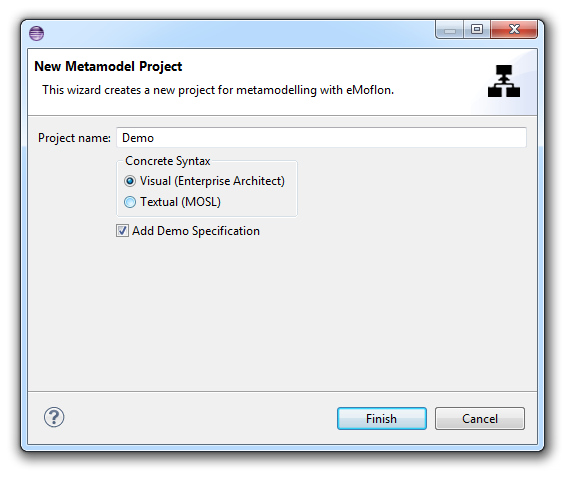
\includegraphics[width=0.9\textwidth]{eclipse_newMetamodelDialog}
	\caption{Choose your syntax}
	\label{fig_chooseSyntax}
\end{figure} 

\vspace{1cm}

% Edit me in the morning? I don't like the way this is written..
\item[$\blacktriangleright$]  Another new action on the toolbar is a button with an ``L'' on it (Fig.~\ref{fig_logger}). A log file is written everytime
you save your file, and appears in the eMoflon console window found below the main editor. This log contains important information for us if anything goes
wrong! You can silence certain loggers, set the level of loggers, and configure other settings\footnote{If you're not sure how to do this, check out a short
Log4j tutorial at \href{http://logging.apache.org/log4j/1.2/manual.html}{http://logging.apache.org/log4j/1.2/manual.html}} by clicking on this button and
modifying the \texttt{log4jConfig.properties} file.

\newpage
\vspace*{3cm}
\begin{figure}[htbp]
	\centering
  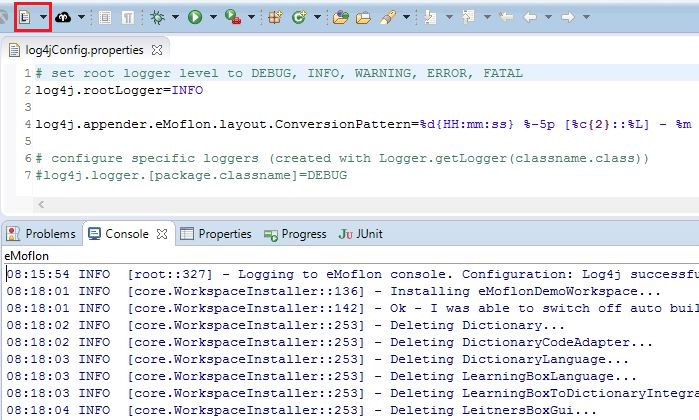
\includegraphics[width=0.9\textwidth]{eclipse_logger}
	\caption{The eMoflon logger}
	\label{fig_logger}
\end{figure} 
\end{itemize}

\fancyfoot[R]{ $\triangleright$ \hyperlink{simpleDemo vis}{Next [visual]\hspace{0.2cm}} \\ $\triangleright$ \hyperlink{simpleDemo tex}{Next [textual]}}

\clearpage
\visHeader

\subsection{A first look at Enterprise Architect}

\begin{itemize}
\FloatBarrier
\hypertarget{simpleDemo vis}{}
\item[$\blacktriangleright$] Can you locate the new \texttt{Demo.eap} file in your package explorer? This is the EA project file you'll be
modelling in. Don't worry any other folders at the moment - all problems will be resolved by the end of this section.

In the meantime, do not rename, move, or delete anything.

\item[$\blacktriangleright$] Double-click \texttt{Demo.eap} to start EA, and choose \texttt{Ultimate} when starting EA for the first time.

\item[$\blacktriangleright$] In EA, navigate to ``Extensions/MOFLON::Ecore Addin/Export\- all\- to\- Workspace'' (Fig.~\ref{fig:ea}). 

\begin{figure}[htbp]
	\centering
  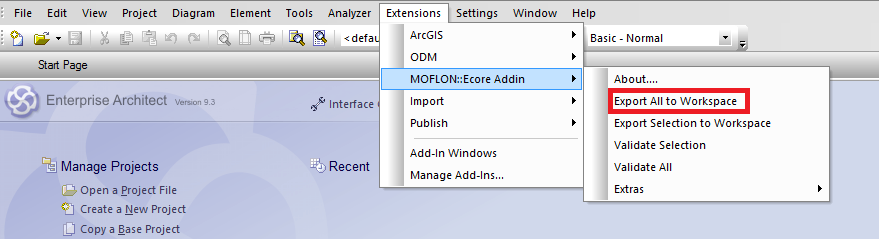
\includegraphics[width=0.9\textwidth]{ea_firststart}
	\caption{Export from EA} 
	\label{fig:ea} 
\end{figure}

\item[$\blacktriangleright$] Please note that this submenu is limited, and does not provide access to all eMoflon functionality. You can activate eMoflon's full
control panel window by going to ``Extensions/Add-In Windows'' (Fig.~\ref{fig:controlPanel}). To export from here, click \texttt{All} in the ``Export'' section.

\begin{figure}[htbp]
	\centering
  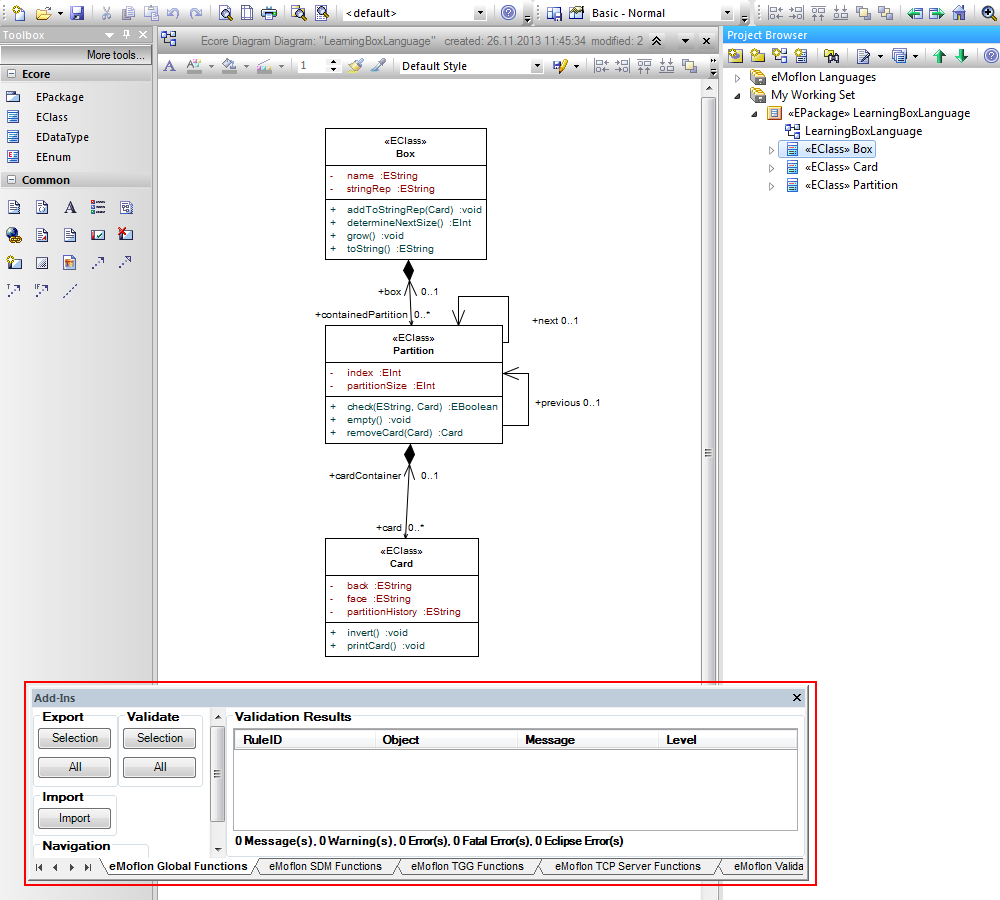
\includegraphics[width=0.9\textwidth]{ea_controlPanel}
	\caption{eMoflon's control panel} 
	\label{fig:controlPanel} 
\end{figure}

\item[$\blacktriangleright$] Now try exploring the EA project browser! Try to navigate to the packages, classes, and diagrams. Don't worry if you don't
understand that much - we'll get to explaining everything in a moment. Just make sure not to change anything!

%\nxtPage{\thepage}
\newpage

\item[$\blacktriangleright$] Switch back to Eclipse, choose your metamodel project, and press F5 to refresh. A new folder should appear, and your errors should
disappear after a few seconds. Since you've chosen to use our visual syntax, there isn't much to look at here. The export from EA places all required files in a
hidden folder(.temp) in the project, and refreshing triggers a build process that invokes our code generator automatically. 

\item[$\blacktriangleright$] You should be able to monitor the progress with the green bar in the lower right corner (Fig.~\ref{fig_eclipseBuild}). Pressing the
symbol opens a monitor view that gives more details of the build process. You don't need to worry about any of these details, just remember to refresh your
Eclipse workspace after an export.

\fancyfoot[OR]{$\triangleright$ \hyperlink{validate common}{Next}}

\begin{figure}[htbp]
	\centering
  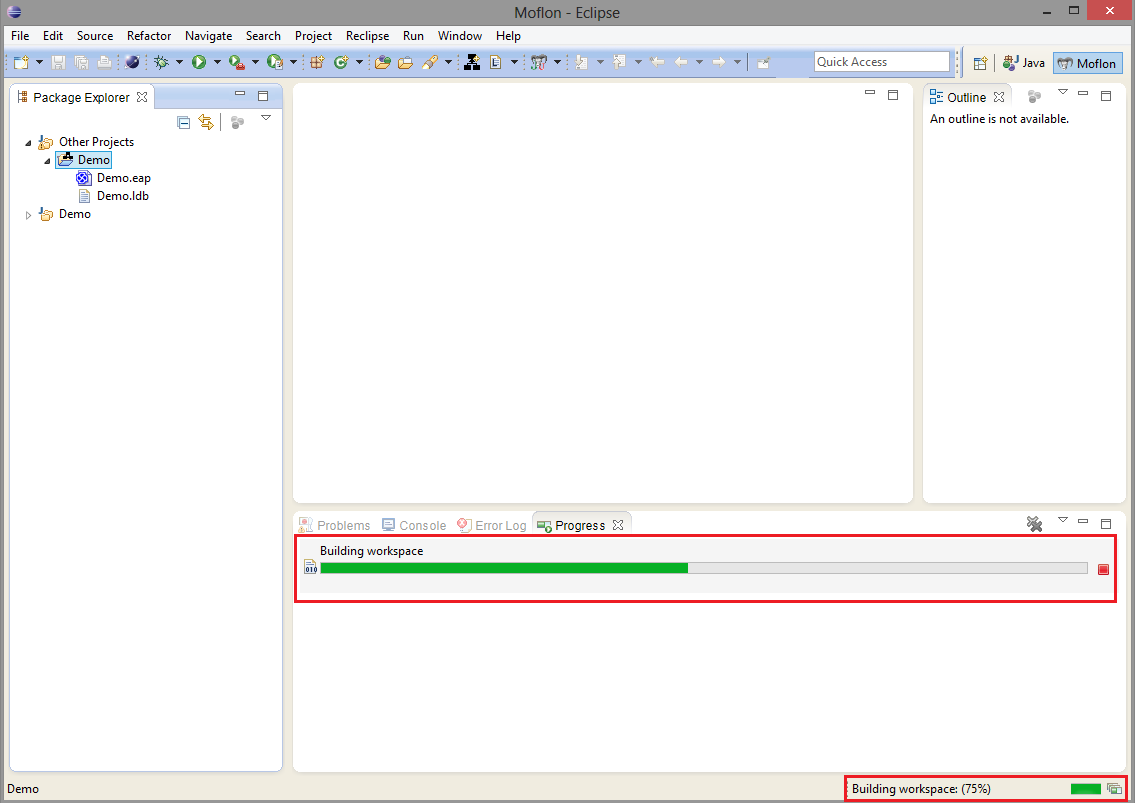
\includegraphics[width=0.9\textwidth]{eclipse_building}
	\caption{Eclipse workspace when using visual syntax} 
	\label{fig_eclipseBuild} 
\end{figure}

\item[$\blacktriangleright$] If you're ever worried about forgetting to refresh your workspace, or if you just don't want to bother with having to do this,
Eclipse does offer an option to do it for you automatically. To activate this, Go to ``Window/Preferences/General/Workspace" and select \texttt{refresh on
access}.

\end{itemize}

\newpage
\texHeader
% \fancyfoot[R]{$\triangleright$ \hyperlink{validate common}{Next}}

\subsection{A first look at MOSL}

\begin{itemize}
\FloatBarrier
\hypertarget{simpleDemo tex}{} 
\item[$\blacktriangleright$] You should immediately have 3 folders available in your project explorer - Your metamodel project,
\texttt{DoubleLinkedListLanguage}, and \\ \texttt{texDemoTestSuite}. Initially, you'll see a red exclamation mark indicating there are errors, but once you give
Eclipse a few seconds to refresh, all problems should be solved.

\item[$\blacktriangleright$] That's it! You're all set up! But, while you're here, feel free to explore the ``Demo'' folder. It has the basic code that implements
this demo, and we recommend you take a brief look to get a feel for the the general syntax.

In the meantime, please do not rename, move, or delete anything.
\end{itemize}


\newpage
\genHeader
\fancyfoot[R]{ $\triangleright$ \hyperlink{projectStructure vis}{Next visual task} \\ $\triangleright$ \hyperlink{projectStructure tex}{Next textual step} }

\section{Validate your installation with JUnit}

\begin{itemize}

\item[$\blacktriangleright$] In\hypertarget{validate common}{} the eclipse workspace, choose ``Working Sets'' as your top level element in the package explorer (Fig.~\ref{fig_topLevel}). We work with many working sets, and use them to structure the workspace in Eclipse.

\begin{figure}[htbp]
	\centering
  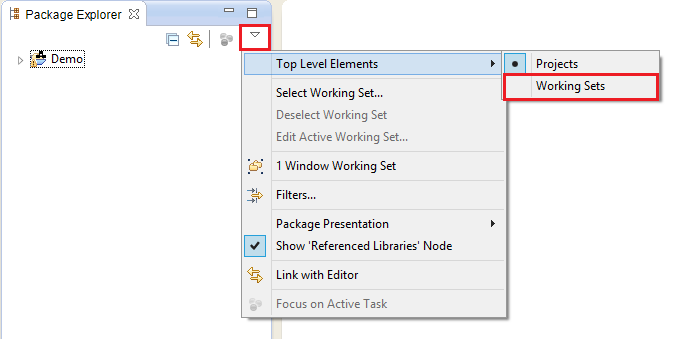
\includegraphics[width=1\textwidth]{eclipse_workingsets}
	\caption{Top Level Elements in Eclipse}
	\label{fig_topLevel}
\end{figure}

\item[$\blacktriangleright$] The files have now been restructured and sorted into three nodes. The organization for these nodes will be explained in a moment but for now, check out ``Other Projects/DemoTestSuite.'' This is the testing unit imported with the demo files to make sure everything was installed and set up correctly. Right click on the Project to bring up the context menu and press ``Run As/JUnit Test.'' If anything goes wrong, try refereshing by choosing folders and pressing  \texttt{F5}, or right-clicking and selecting ``Refresh.''

\vspace{0.5cm}

\begin{figure}[htbp]
	\centering
  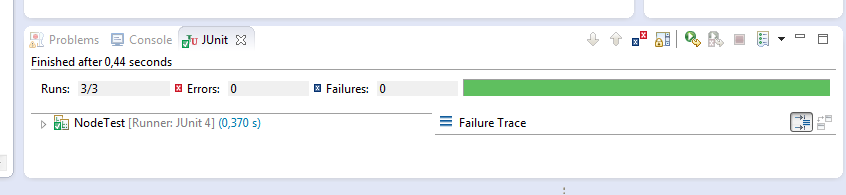
\includegraphics[width=1\textwidth]{eclipse_passedJUnitTest}
	\caption{All's well that ends well\ldots}
	\label{fig_passedTest}
\end{figure}

\vspace{0.5cm}

Congratulations!  If you see a green bar  (Fig.~\ref{fig_passedTest}), then everything has been set up correctly and you are now ready to start metamodelling!

\end{itemize}

\newpage
\section{Project setup}

% No new page; first page call under this section. see ProjectStructureSrc . 
\genHeader

\subsection{Your Enterprise Architect Workspace}

Now\hypertarget{projectStructure vis}{} that everything is installed and setup properly, let's take a closer look at the different workspaces and our workflow.
Before we continue, please make a few slight adjustments to Enterprise Architect (EA) so you can easily compare your current workspace to our screenshots.
These settings are advisable but you are, of course, free to choose your own colour schema.

\begin{stepbystep}

\item  Select \menuPath{Tools \menuSep Options \menuSep Themes} in EA, and set Diagram Theme to \texttt{Enterprise Architect 10}.

\item  Next, proceed to \menuPath{Gradients and Background} and set \menuPath{Gradient} and \menuPath{Fill} to \entity{White} (\Cref{ea:paperAndElementFill}). 

\begin{figure}[htbp]
    \centering
    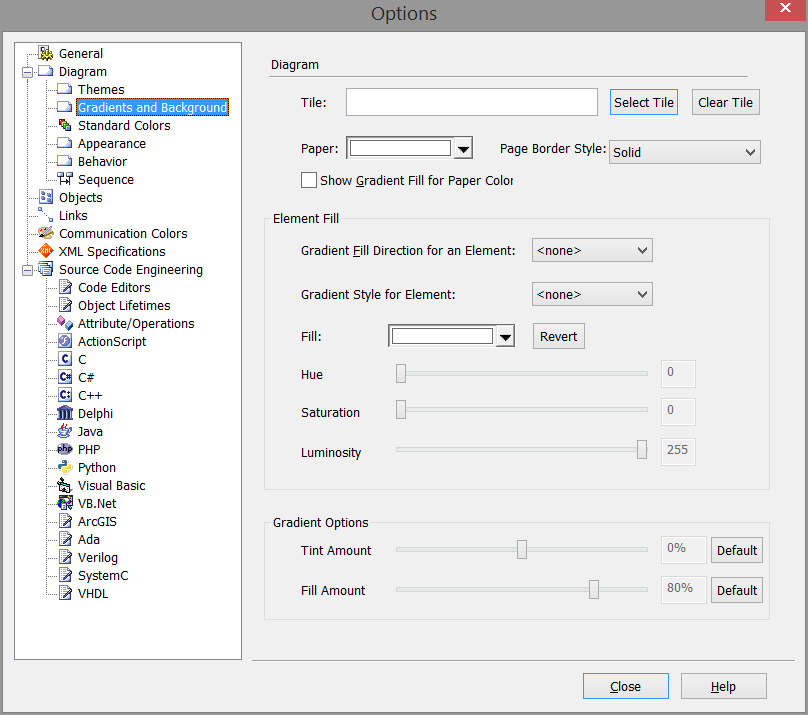
\includegraphics[width=0.8\textwidth]{standardPaperAndFill}
    \caption{Suggested paper background and element fill}
    \label{ea:paperAndElementFill}
\end{figure}

\item  In the \menuPath{Standard Colors} tab, and set your colours to reflect \Cref{ea:standardColoursEA}.

\begin{figure}[htbp]
  \centering
  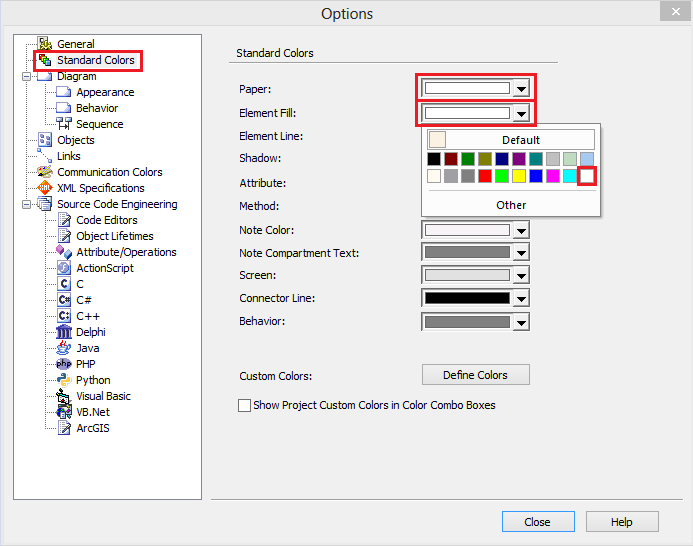
\includegraphics[width=0.8\textwidth]{standardColours}
  \caption{Our choice of standard colours for diagrams in EA}
  \label{ea:standardColoursEA}
\end{figure}

\vspace{0.5cm}

\item 
In the same dialogue, go to \menuPath{Diagram \menuSep Appearance} and reflect the settings in \Cref{ea:standardAppearanceEA}.
Again, this is just a suggestion and not mandatory.

\item 
Last but not least open the \menuPath{Code Engineering} toolbar (\Cref{ea:standardSCEEA1}) and choose \entity{Ecore} as the default language (\Cref{ea:standardSCEEA2}).
\textbf{This setting is mandatory, and very important.}
\end{stepbystep}

\begin{figure}[htbp]
  \centering
  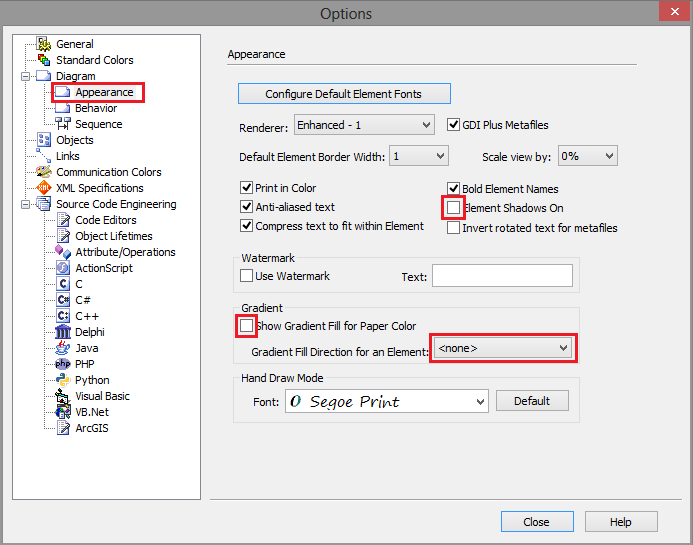
\includegraphics[width=0.8\textwidth]{standardAppearance}
  \caption{Our choice of the standard appearance for model elements}
  \label{ea:standardAppearanceEA}
\end{figure}

\begin{figure}[htbp]
    \centering
    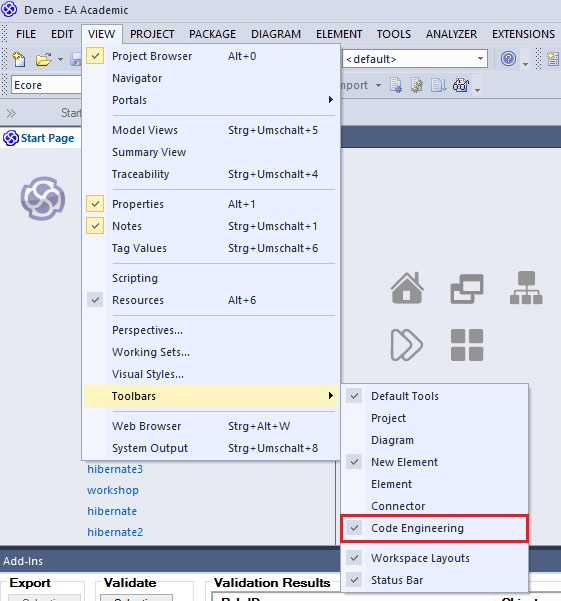
\includegraphics[width=0.8\textwidth]{standardCodeEngineering1}
    \caption{Open the \menuPath{Code Engineering} toolbar}
    \label{ea:standardSCEEA1}
 \end{figure}

\begin{figure}[htbp]
    \centering
    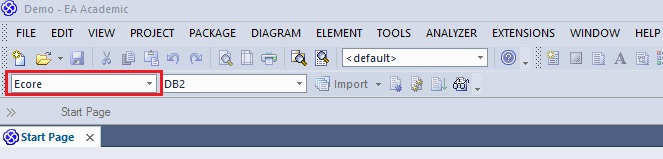
\includegraphics[width=0.8\textwidth]{standardCodeEngineering2}
    \caption{Make sure you set the standard language to \entity{Ecore}}
    \label{ea:standardSCEEA2}
 \end{figure}
 
\clearpage

In your EA \enquote{workspace} (actually referred to as an \emph{EA project}), take a careful look at the project browser:
The root node \texttt{Demo} is called a \emph{model} in EA lingo, and is used as a container to group a set of related \emph{packages}.
In our case, \texttt{Demo} contains a single package \texttt{org.moflon.demo.doublelinkedlist}.
An EA project however, can consist of numerous models that in turn, group numerous packages.

Now switch back to your Eclipse workspace and note the two nodes named \texttt{Specifications} and \texttt{org.moflon.demo} (\Cref{eclipse:eclipsePS}).

\begin{figure}[htbp]
    \centering
    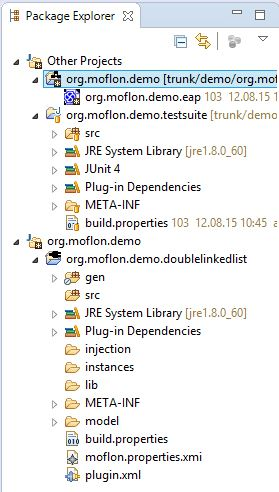
\includegraphics[width=0.4\textwidth]{eclipse_visPackageExplorer}
    \caption{Project structure}
    \label{eclipse:eclipsePS}
 \end{figure}

These nodes, used to group related \emph{Eclipse projects} in an Eclipse workspace, are called \emph{working sets}. The working set
\texttt{Spe\-ci\-fi\-ca\-tions} contains all \emph{metamodel projects} in a  workspace. Your metamodel project contains a single EAP (EA project) file and is
used to communicate with EA and initiate code generation by simply pressing \texttt{F5} or choosing \texttt{Refresh} from the context menu. In our case,
\texttt{Specifications} should contain a single metamodel project \texttt{org.moflon.demo} containing our EA project file \texttt{org.moflon.demo.eap}.
 
\Cref{fig:fromEAtoEclipse} depicts how the Eclipse working set \texttt{org.moflon.demo} and its contents were generated from the EA model \texttt{org.moflon.demo}. Every model
in EA is mapped to a working set in Eclipse with the same name. From every package in the EA model, an Eclipse project is generated, also with the same name.
%\LK{Fix names and screenshot (does not match previous figure)}

\begin{figure}[htbp]
    \centering
  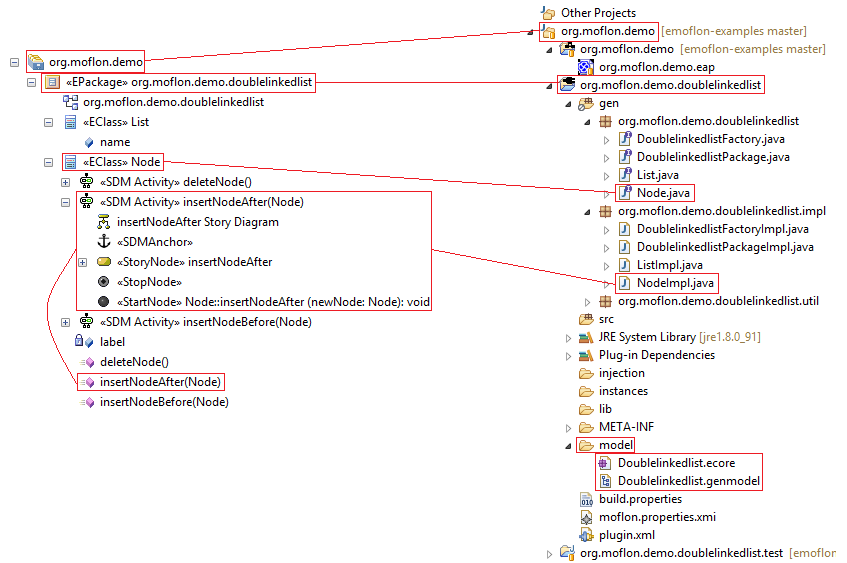
\includegraphics[width=\textwidth]{fromEAToEclipse}
    \caption{Mapping between artefacts in EA and Eclipse}
    \label{fig:fromEAtoEclipse}
\end{figure}

These projects, however, are of a different nature than, for example, metamodel projects or normal Java projects.
These are called \emph{repository projects}.
A \newconcept{nature} is Eclipse lingo for \enquote{project type} and is visually indicated by a corresponding nature icon on the project folder.
Our metamodel projects sport a neat little class diagram symbol.
Repository projects are generated automatically with a certain project structure according to our conventions.

The \entity{model} subfolder in the Eclipse package explorer is probably the most important as it contains the \newconcept{Ecore model} for the project. Ecore is a metamodeling language that provides building blocks such as \newconcept{classes} and \newconcept{references} for defining the static structure (concepts and relations between concepts) of a system.
This folder also contains a \newconcept{genmodel}, the second model required by the Eclipse Modeling Framework (EMF) to generate Java code.

Looking back to \Cref{fig:fromEAtoEclipse}, realize that it also depicts how the class \entity{Node} in the EA model is mapped to the Java interface \entity{Node}.
Double-click \entity{Node.java} and take a look at the methods declared in the interface. These correspond directly to the methods declared in the modeled \entity{Node} class.

As indicated by the source folders \entity{src}, \entity{injection}, and \entity{gen}, we advocate a clean separation of hand-written (should be placed in \entity{src} and \entity{injection}) and generated code (automatically in \texttt{gen}).
As we shall see later in the handbook, hand-written code can be
integrated in generated classes via \emph{injections}.
This is sometimes necessary for small helper functions.

Have you noticed the methods of the \entity{Node} class in our EA model? 
Now hold on tight---each method can be \newconcept{modeled} completely in EA and the corresponding implementation in Java is generated automatically and placed in \texttt{NodeImpl.java}.
Just in case you didn't get it: The behavioural or dynamic aspects of a system can be completely modeled in an abstract, platform-/programming language--independent fashion using a blend of activity diagrams and a \enquote{graph pattern} language called \newconcept{Story~Driven~Modelling}~(SDM).
In our EA project, these \newconcept{Story Diagrams} or simply \emph{SDM}s, are placed in \newconcept{SDM Containers} named according to the method they implement.
For instance, \texttt{\guillemotleft{}SDM Activity\guillemotright{} insertNodeAfter SDM} for the method \texttt{in\-sert\-NodeAft\-er(Node)} as depicted in \Cref{fig:fromEAtoEclipse}.
We'll dedicate Part III of the handbook to understanding why SDMs are so  {\huge crazily} cool!

To recap all we've discussed, let's consider the complete workflow as depicted in \Cref{fig:Overview}. We started with a concise model in EA, simple and
independent of any platform specific details~(1).  Our EA model consists not only of static aspects modelled as a class diagram~(2), but also of dynamic aspects
modelled using SDM~(3).  After exporting the model and code generation~(4), we basically switch from \emph{modelling} to \emph{programming} in a specific
general purpose programming language (Java). On this lower \emph{level of abstraction}, we can flesh out the generated repository~(5) if necessary, and mix as
appropriate with hand-written code and libraries.  Our abstract specification of behaviour (methods) in SDM is translated to a series of method calls that form
the body of the corresponding Java method~(6).

\begin{figure}[htbp]
	\centering
  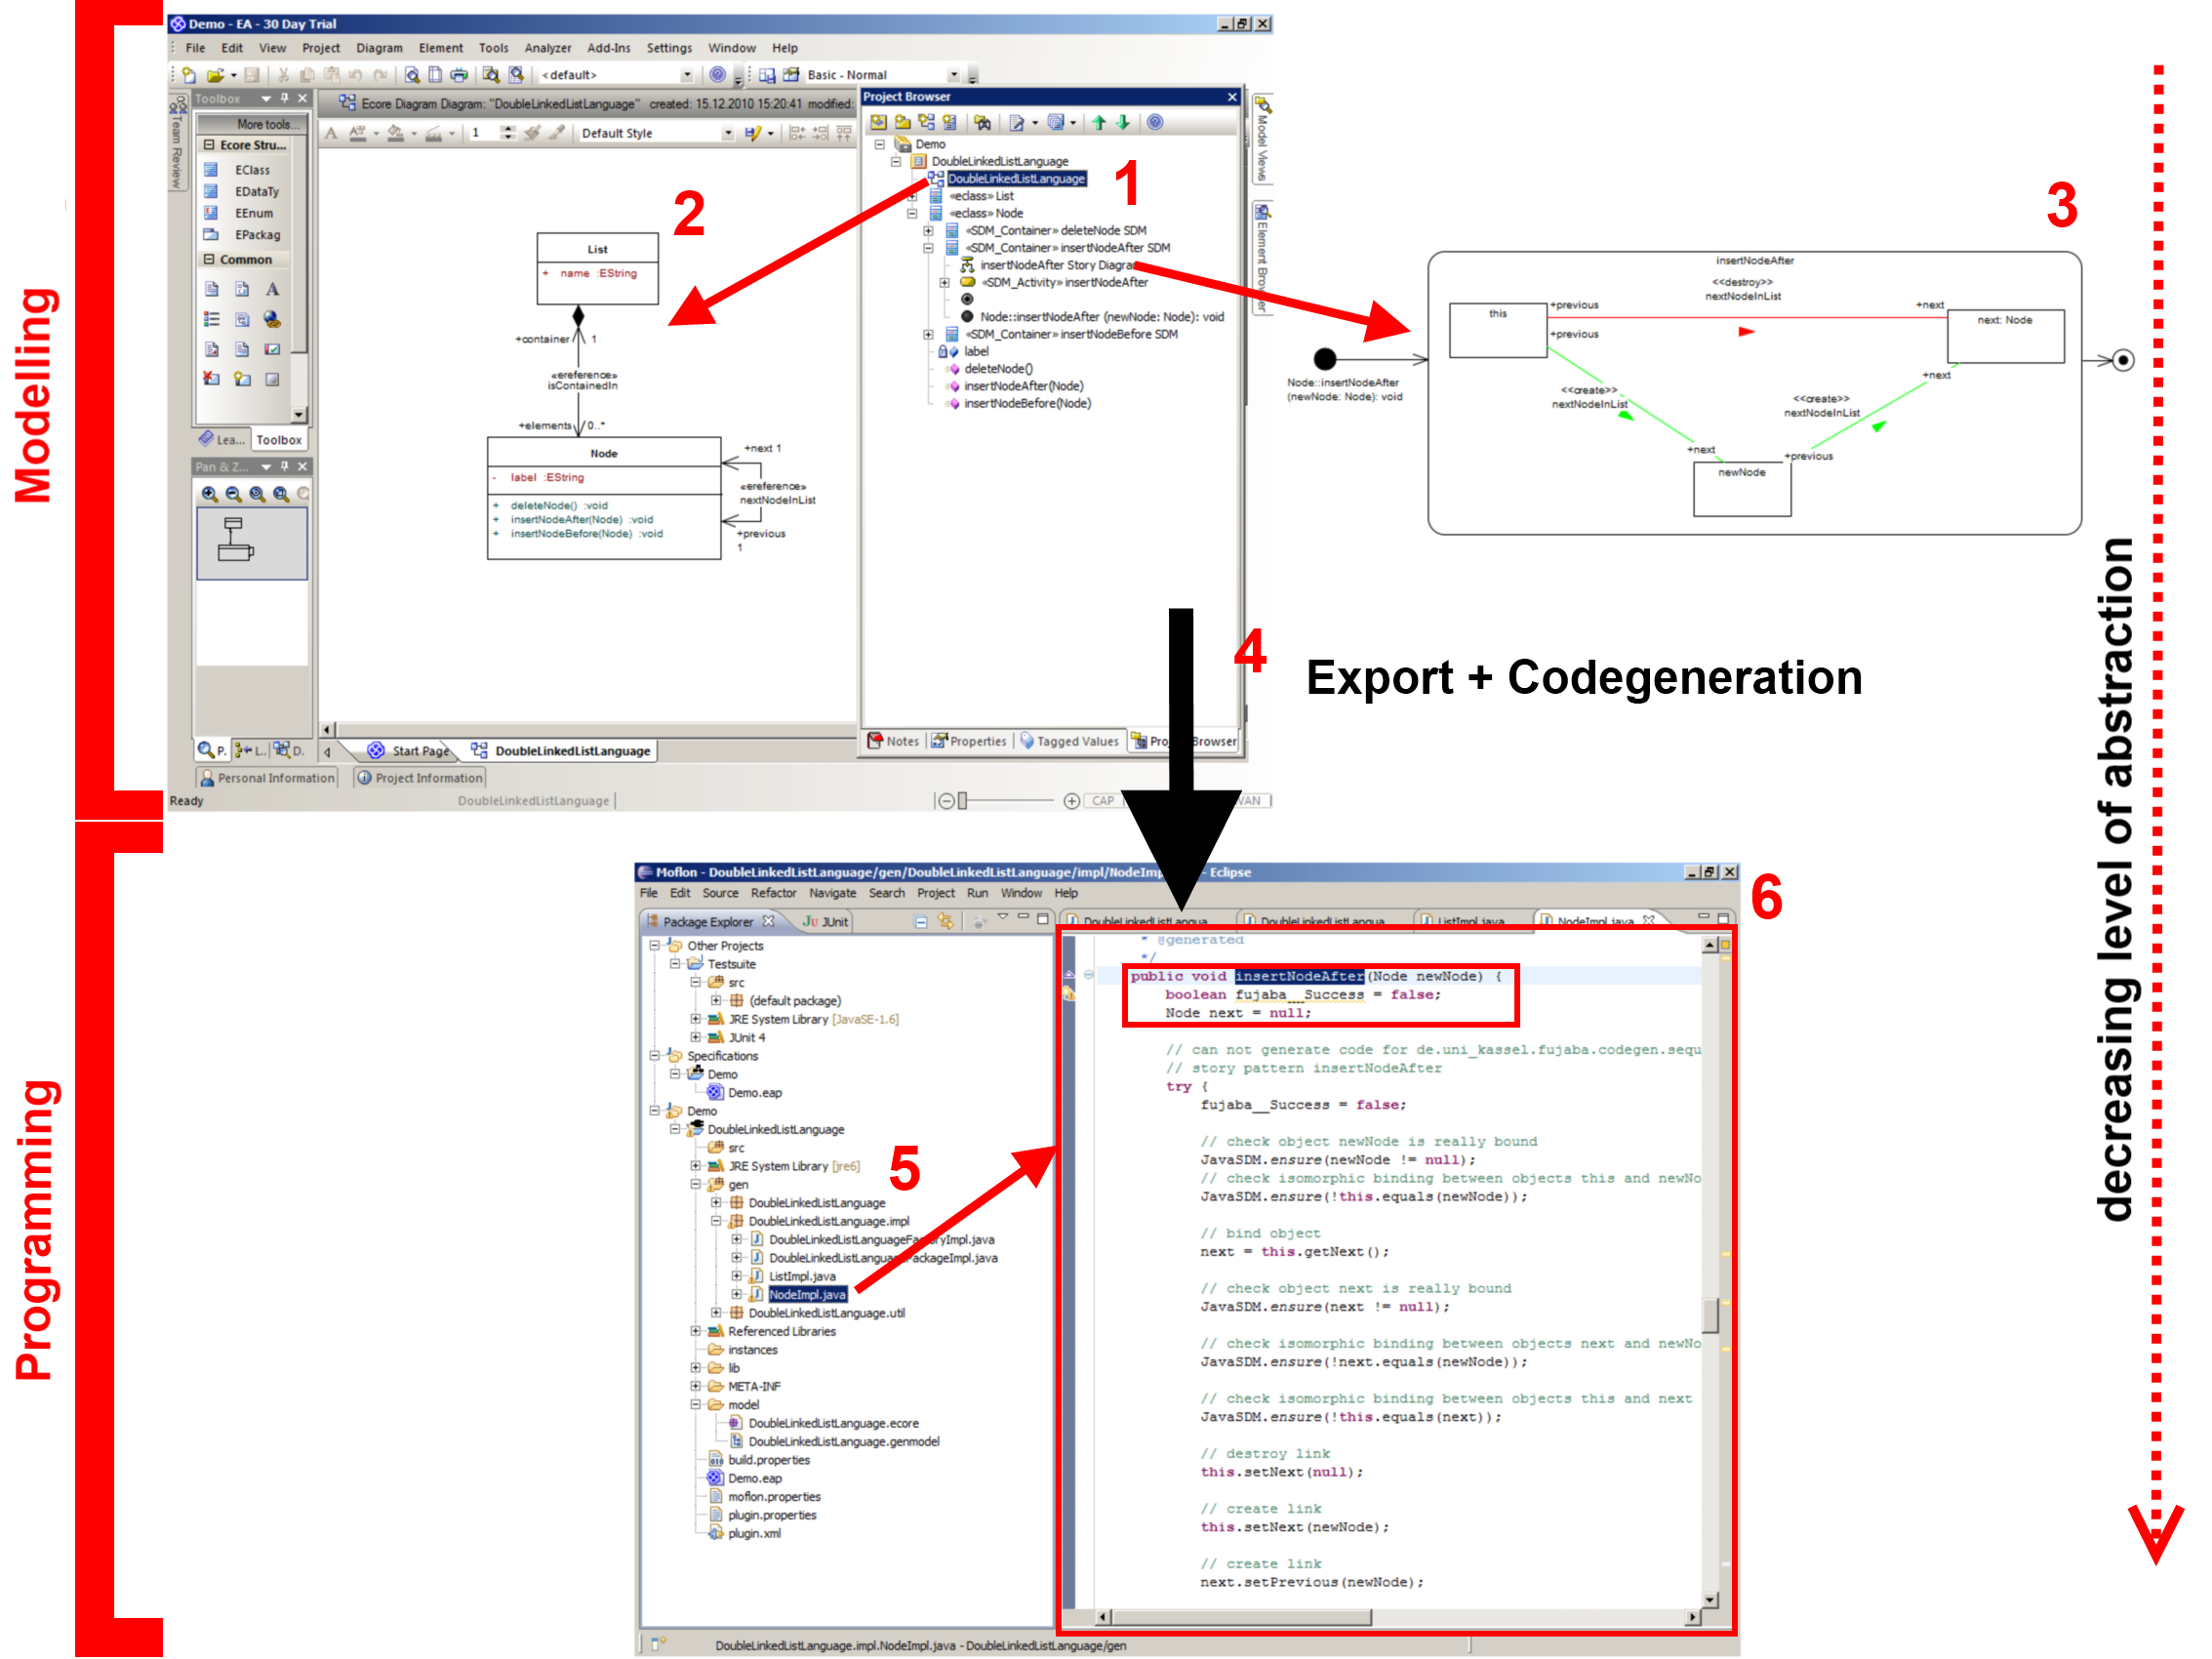
\includegraphics[width=1.1\textwidth]{tafelbild}
	\caption{Overview}
	\label{fig:Overview}
\end{figure}


\clearpage

\newpage
\genHeader
\hypertarget{codeGen common}{} 
\chapter{Generated code vs. hand-written code}

Now that you've worked through the specifics of your syntax, lets have a brief discussion on code generation.

The Ecore model is used to drive a code generator that maps the model to Java interfaces and classes. The generated Java code that represents the model is often
referred to as a repository. This is the reason why we refer to such projects as repository projects. A repository can be viewed as an adapter that enables
building and manipulating concrete instances of a specific model via a programming language such as Java. This is why we indicate repository projects using a
cute adapter/plug symbol on the project folder.

If you take a careful look at the code structure in \texttt{gen} (\Cref{eclipse:structureGen}), you'll find a \texttt{FooImpl.java} for every
\texttt{Foo.java}. Indeed, the subpackage \texttt{.impl} contains Java classes that implement the interfaces in the parent package. Although this might strike
you as unnecessary (why not merge interface and implementation for simple classes?), this consequent separation in interfaces and implementation allows for a
clean and relatively simple mapping of Ecore to Java, even in tricky cases such as multiple inheritance (allowed and very common in Ecore models). A further
package \texttt{.util} contains some auxiliary classes such as a factory for creating instances of the model.

 \begin{figure}[htbp]
  \centering
  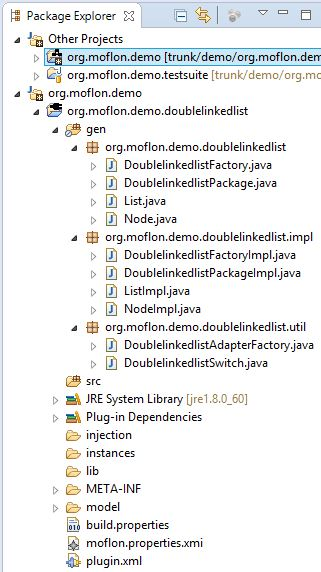
\includegraphics[width=0.4\textwidth]{../../org.moflon.doc.handbook.01_installation/5_codeGeneration/eclipse_structureGen}
  \caption{Package structure of generated code (\texttt{gen})}
  \label{eclipse:structureGen}
\end{figure}

If this is your first time of seeing generated code, you might be shocked at the sheer amount of classes and code generated from our relatively simple model.
You might be thinking: ``Hey -- if I did this by hand, I wouldn't need half of all this stuff!''  Well, you're right and you're wrong. The point is that an
automatic mapping to Java via a code generator scales quite well.

This means for simple, trivial examples (like our double linked list), it might be possible to come up with a leaner and simpler Java representation. For
complex, large models with lots of mean pitfalls however, this becomes a daunting task. The code generator provides you with years and \emph{years} of
experience of professional programmers who have thought up clever ways of handling multiple inheritance, an efficient event mechanism, reflection, consistency
between bidirectionally linked objects, and much more.

A point to note here is that the mapping to Java is obviously not unique. Indeed there exist different standards of how to map a modelling language to a
general purpose programming language such as Java. As previously mentioned, we use a mapping defined and implemented by the Eclipse Modelling Framework (EMF),
which tends to favour efficiency and simplicity over expressiveness and advanced features.
 

% References?
%

% Glossary?
%

\end{document}